\documentclass[11pt,a4paper,oneside]{report}

% Page Geometry
\usepackage[a4paper,top=2.5cm,bottom=2.5cm,left=2.5cm,right=2.5cm,headheight=14pt]{geometry}

% Typography and Language
\usepackage{microtype}

% Mathematical Formatting
\usepackage{amsmath,amssymb,amsthm}

% Tables and Formatting
\usepackage{booktabs}
\usepackage{longtable}
\usepackage{array}
\usepackage{multirow}
\usepackage{makecell}
\usepackage{float}
\usepackage{caption}

% Lists
\usepackage{enumitem}
\setlist{topsep=2pt,partopsep=0pt,parsep=1pt,itemsep=2pt}

% Colors
\usepackage{xcolor}
\definecolor{primaryblue}{RGB}{26, 82, 118}
\definecolor{secondaryblue}{RGB}{41, 128, 185}
\definecolor{darkslate}{RGB}{44, 62, 80}
\definecolor{lightgray}{RGB}{245, 247, 250}
\definecolor{bordergray}{RGB}{200, 205, 210}
\definecolor{codebackground}{RGB}{248, 249, 250}
\definecolor{commentgreen}{RGB}{39, 174, 96}
\definecolor{stringred}{RGB}{192, 57, 43}
\definecolor{keywordblue}{RGB}{41, 128, 185}
\definecolor{forestgreen}{RGB}{34, 139, 34}
\definecolor{warningamber}{RGB}{214, 137, 16}
\definecolor{dangerred}{RGB}{192, 57, 43}

% Code Listings
\usepackage{listings}
\lstdefinelanguage{json}{
    basicstyle=\ttfamily\footnotesize,
    showstringspaces=false,
    breaklines=true,
    frame=single,
    stringstyle=\color{stringred},
    commentstyle=\color{commentgreen}
}
\lstdefinelanguage{JavaScript}{
    keywords={typeof, new, true, false, catch, function, return, null, switch, var, if, in, while, do, else, case, break, const, let, export, default, from, import},
    keywordstyle=\color{keywordblue}\bfseries,
    identifierstyle=\color{black},
    sensitive=false,
    comment=[l]{//},
    morecomment=[s]{/*}{*/},
    commentstyle=\color{commentgreen}\ttfamily,
    stringstyle=\color{stringred}\ttfamily,
    morestring=[b]',
    morestring=[b]"
}
\lstset{
    backgroundcolor=\color{codebackground},
    basicstyle=\ttfamily\footnotesize,
    breakatwhitespace=false,
    breaklines=true,
    captionpos=b,
    commentstyle=\color{commentgreen},
    keepspaces=true,
    keywordstyle=\color{keywordblue}\bfseries,
    numbers=left,
    numbersep=7pt,
    numberstyle=\tiny\color{darkgray},
    showspaces=false,
    showstringspaces=false,
    showtabs=false,
    stringstyle=\color{stringred},
    tabsize=2,
    frame=single,
    rulecolor=\color{bordergray},
    xleftmargin=15pt,
    framexleftmargin=15pt
}

% TikZ & Graphics
\usepackage{tikz}
\usetikzlibrary{shapes.geometric,arrows.meta,positioning,calc,fit,backgrounds}

% Headers and Footers
\usepackage{fancyhdr}
\pagestyle{fancy}
\fancyhf{}
\fancyhead[L]{\textcolor{darkslate}{\small\slshape\leftmark}}
\fancyhead[R]{\textcolor{darkslate}{\small I-ITSM Final Project Report}}
\fancyfoot[C]{\textcolor{darkslate}{\thepage}}
\renewcommand{\headrulewidth}{0.4pt}
\renewcommand{\footrulewidth}{0.4pt}

% Hyperlinks
\usepackage{hyperref}
\hypersetup{
    colorlinks=true,
    linkcolor=primaryblue,
    citecolor=forestgreen,
    urlcolor=secondaryblue,
    bookmarksnumbered=true,
    pdfauthor={Anay Goenka, Anshul Naik, Krish Jain, Anirudh Yendalur},
    pdftitle={I-ITSM: Intelligent IT Service Management System - Final Project Report},
    pdfsubject={Multi-Module ITIL Incident Management with Algorithmic Assignment and SLA Governance}
}

% Custom Command Definitions
\newcommand{\moduleone}{\textbf{M1 (Identity \& Access Management)}}
\newcommand{\moduletwo}{\textbf{M2 (Incident Management)}}
\newcommand{\modulethree}{\textbf{M3 (Technician Management \& Assignment)}}
\newcommand{\modulefour}{\textbf{M4 (SLA, Audit \& Notifications)}}

\newcolumntype{L}[1]{>{\raggedright\arraybackslash}p{#1}}
\newcolumntype{C}[1]{>{\centering\arraybackslash}p{#1}}
\newcolumntype{R}[1]{>{\raggedleft\arraybackslash}p{#1}}


\begin{document}

% Title Page
\begin{titlepage}
    \centering
    \vspace*{1.5cm}
    
    {\Huge \bfseries \textcolor{primaryblue}{I-ITSM: Intelligent IT Service\\Management System}}\\[0.8cm]
    {\Large \bfseries \textcolor{darkslate}{A Multi-Module ITIL-Compliant Incident Management Platform\\with Algorithmic Technician Assignment and Automated SLA Governance}}\\[1.5cm]
    
    \rule{\linewidth}{1.2pt}\\[0.6cm]
    {\large \textbf{Comprehensive Architectural, Implementation, and Verification Final Report}}\\[0.6cm]
    \rule{\linewidth}{1.2pt}\\[2.0cm]
    
    \begin{minipage}{0.85\textwidth}
    \centering
    \textbf{\Large Project Engineering Authorship \& Module Ownership:}\\[0.6cm]
    \begin{tabular}{ll}
        \textbf{Anay Goenka} & \textit{Module 1: Identity, Platform \& Access Management} \\
        \textbf{Anshul Naik} & \textit{Module 2: Incident Management \& Lifecycle Engine} \\
        \textbf{Krish Jain} & \textit{Module 3: Technician Management \& Algorithmic Assignment} \\
        \textbf{Anirudh Yendalur} & \textit{Module 4: SLA Tracking, Audit Logging \& Notifications} \\
    \end{tabular}
    \end{minipage}\\[2.5cm]
    
    \vfill
    {\large \textbf{Academic \& Technical Final Submission}}\\[0.3cm]
    {\normalsize Department of Computer Science \& Information Technology}\\[0.2cm]
    {\normalsize November 2026}
\end{titlepage}

% Abstract
\cleardoublepage
\phantomsection
\addcontentsline{toc}{chapter}{Abstract}
\chapter*{Abstract}
Modern enterprise IT infrastructures demand resilient, automated, and strictly governed IT Service Management (ITSM) solutions capable of handling high-volume operational incidents with minimal mean time to resolution (MTTR). Traditional ITSM workflows frequently suffer from fragmented triage, arbitrary ticket dispatching, skill-workload mismatches, and delayed service level agreement (SLA) breach responses. 

This comprehensive technical report presents the architectural design, algorithmic underpinnings, implementation details, and empirical validation of the \textbf{Intelligent IT Service Management System (I-ITSM)}. I-ITSM is engineered as a high-performance Layered Modular Monolith adhering to the ITIL v4 framework, comprising four decoupled, highly integrated functional modules:
\begin{itemize}[leftmargin=1.5cm]
    \item \textbf{Module 1 (Identity \& Access Management - Anay Goenka):} Delivers cryptographically secured role-based authentication, user account governance, IT service catalogue tracking, and executive key performance indicators.
    \item \textbf{Module 2 (Incident Management - Anshul Naik):} Implements an immutable-code incident lifecycle state machine, deterministic priority scoring ($P1$ to $P4$), trigram-based duplicate similarity detection, ticket merging, and soft-archiving.
    \item \textbf{Module 3 (Technician Management \& Assignment - Krish Jain):} Operates a multi-dimensional technician competency engine featuring skill proficiency matrices, real-time workload tracking, deterministic multi-criteria assignment algorithms (Skill-Based and Least-Loaded), and optional LLM-assisted recommendation reasoning with guaranteed fallback.
    \item \textbf{Module 4 (SLA, Audit \& Notifications - Anirudh Yendalur):} Executes real-time SLA policy tracking via an asynchronous 60-second periodic daemon, automated 80\% warning thresholds, instant breach alerts, in-app notification routing with real-time polling, and an append-only immutable audit trail.
\end{itemize}

The platform is realized through a modern asynchronous technology stack powered by Python FastAPI, SQLAlchemy 2.0 Asyncio with Psycopg 3, PostgreSQL 16+, and a React 18 Single-Page Application featuring customized design tokens, centralized error parsing, and a strict Zero-UUID presentation paradigm. Rigorous verification across 273 automated tests spanning unit, integration, and API layers confirms complete functional correctness, transactional integrity, and zero regressions.

\vspace{0.8cm}
\noindent\textbf{Keywords:} IT Service Management, ITIL v4, Incident Lifecycle, Algorithmic Assignment, SLA Governance, Modular Monolith, FastAPI, React, PostgreSQL.

% Executive Summary
\cleardoublepage
\phantomsection
\addcontentsline{toc}{chapter}{Executive Summary}
\chapter*{Executive Summary}
Information Technology Service Management (ITSM) constitutes the operational backbone of digital enterprises. Operational outages, hardware failures, database query timeouts, and network degradations directly jeopardize revenue generation and business continuity. Industry benchmarks indicate that manual incident classification and assignment consume upwards of 35\% of ticket lifecycle duration, leading to substantial SLA violation penalties and operational bottlenecks.

The \textbf{I-ITSM Platform} addresses these enterprise challenges by establishing an automated, reliable, and auditable incident orchestration ecosystem. Across a rigorous multi-month engineering effort, our team established clear architectural boundaries and developed four core modules with complete functional synergy:

\begin{enumerate}
    \item \textbf{Automated Triage and Priority Scoring:} Rather than relying on subjective human assessment, I-ITSM calculates ticket priority deterministically using a weighted multi-variable matrix:
    \[
    \text{Score} = 0.4 \times \text{Impact} + 0.4 \times \text{Urgency} + 0.2 \times \text{Business Criticality}
    \]
    This ensures that high-impact incidents affecting mission-critical business services immediately receive $P1$ (Critical) status.
    
    \item \textbf{Smart Algorithmic Assignment:} The assignment engine evaluates active candidate pools against incident requirements. Utilizing the Strategy Pattern, the system provides both \textit{Skill-Based} matching (weighting skill proficiency by $20\times$ and experience by $2\times$) and \textit{Least-Loaded} balancing. Concurrency protection via Compare-and-Swap (CAS) ensures technician capacity limits are strictly respected under concurrent assignment requests.
    
    \item \textbf{Proactive SLA Governance:} A scheduled background monitor evaluates open incidents against tiered SLA policies every 60 seconds. When an incident reaches 80\% of its target response or resolution deadline, an automated warning is dispatched, enabling technicians and managers to intervene prior to breach.
    
    \item \textbf{Enterprise Usability and Audit Compliance:} The frontend application enforces a Zero-UUID design architecture, replacing raw database identifiers with intuitive incident codes (\texttt{INC-xxxxxxxx}), usernames, and skill badges. Every state change, assignment, and configuration update is logged into an append-only audit ledger.
\end{enumerate}

Empirical evaluation demonstrates 100\% operational test pass rates across 273 test scenarios, sub-second API execution latencies, and flawless multi-role browser end-to-end user workflows.

% Table of Contents, Lists
\cleardoublepage
\tableofcontents

\cleardoublepage
\listoffigures

\cleardoublepage
\listoftables

\cleardoublepage


\chapter{Introduction}
\label{ch:introduction}

\section{Context and Background}
\label{sec:intro_context}
In contemporary enterprise environments, the uninterrupted availability of Information Technology (IT) services is critical to business continuity, regulatory compliance, and customer satisfaction. The Information Technology Infrastructure Library (ITIL) v4 framework defines an \textit{incident} as ``an unplanned interruption to a service or reduction in the quality of a service.'' Effective Incident Management aims to restore normal service operation as rapidly as possible, minimize adverse business impact, and maintain agreed-upon service levels.

Historically, organizations relied on manual ticketing systems, email chains, or spreadsheets to record and track operational disruptions. As enterprise IT environments transitioned toward complex distributed architectures---encompassing microservices, cloud-native deployments, relational and non-relational persistence layers, and hybrid networking topologies---the velocity and volume of incident reports expanded exponentially. 

Manual incident management practices exhibit severe structural deficiencies:
\begin{enumerate}
    \item \textbf{Subjective and Inconsistent Triage:} When end users or tier-1 support agents manually assign priority levels, subjective human biases frequently lead to misclassification. A low-urgency personal peripheral glitch may be tagged as critical, whereas a latent database replication lag affecting high-volume payment processing might be logged with standard priority.
    \item \textbf{Arbitrary Ticket Dispatching:} Support desk coordinators frequently dispatch tickets based on ad-hoc intuition, leading to severe workload imbalances. Seasoned senior technicians become overwhelmed with repetitive triage, while specialized engineers remain idle.
    \item \textbf{Reactive SLA Management:} Traditional systems treat Service Level Agreements (SLAs) as static deadlines evaluated post-resolution. Without active threshold warnings, support teams only recognize an SLA failure after a breach has already materialized, incurring customer penalties and contractual liabilities.
    \item \textbf{Fragmented Auditing and Siloed Communication:} When incident notes, status changes, and technician reassignment histories are not captured in an immutable, centralized ledger, compliance reviews become arduous and error-prone.
\end{enumerate}

\section{Problem Statement}
\label{sec:intro_problem}
To address these enterprise challenges, modern organizations require an automated, intelligent, and architecturally resilient IT Service Management platform. Specifically, the engineering problem tackled in this project involves designing and implementing a system that satisfies four interconnected technical requirements:
\begin{itemize}
    \item \textbf{Identity and Access Isolation:} Enforcing strict Role-Based Access Control (RBAC) across distinct enterprise personas (Employees, Technicians, and Administrators) while maintaining secure token issuance and centralized service catalogs.
    \item \textbf{Lifecycle and Priority Determinism:} Enforcing a formal forward-progressing state machine for incident progression, combined with a deterministic, multi-variable priority scoring algorithm that incorporates impact, urgency, and underlying business service criticality.
    \item \textbf{Competency-Driven Algorithmic Assignment:} Developing extensible assignment algorithms that objectively rank technicians based on categorized technical skills, verified proficiency levels (1 to 5), and active ticket workloads, while guaranteeing capacity headroom constraints under concurrent assignment requests.
    \item \textbf{Automated SLA Governance and Auditability:} Implementing background daemon monitoring capable of preemptively alerting stakeholders when tickets approach 80\% of allowable response or resolution windows, coupled with an immutable event-driven audit ledger and real-time user notification delivery.
\end{itemize}

\section{Project Motivation and Objectives}
\label{sec:intro_objectives}
The primary objective of the \textbf{I-ITSM (Intelligent IT Service Management)} project is the design, development, and verification of a production-grade, ITIL-aligned Incident Management system. The core engineering goals include:

\begin{enumerate}
    \item \textbf{Architectural Modularity and Decoupling:} Design the platform as a Layered Modular Monolith adhering to clean Domain-Driven Design (DDD) principles. The system cleanly segregates four functional modules (M1, M2, M3, and M4) with clear ownership boundaries and an asynchronous, in-process event bus for decoupled side-effects.
    \item \textbf{Algorithmic Incident Triage and Duplicate Suppression:} Implement a mathematical priority matrix calculator and a natural language trigram similarity detector to identify and merge redundant duplicate tickets.
    \item \textbf{Multi-Criteria Assignment Engine:} Provide pluggable assignment strategies (Skill-Based and Least-Loaded) utilizing the Strategy and Factory design patterns, with optional Large Language Model (LLM) reasoning augmentation and robust fallback mechanics.
    \item \textbf{Zero-UUID User Experience Paradigm:} Build an intuitive, responsive frontend Single-Page Application (SPA) in React 18, ensuring that no technical database UUIDs are ever surfaced to end users, replacing them with formatted ticket identifiers (\texttt{INC-xxxxxxxx}), usernames, and semantic badges.
    \item \textbf{Comprehensive Quality Assurance:} Validate 100\% of business rules, security boundaries, and concurrency constraints through an automated test suite exceeding 260 test cases.
\end{enumerate}

\section{Scope of the System}
\label{sec:intro_scope}
The scope of the I-ITSM implementation encompasses:
\begin{itemize}
    \item \textbf{In-Scope Capabilities:}
    \begin{itemize}
        \item User registration, JWT-based authentication, and RBAC policy enforcement for Employee, Technician, and Administrator roles.
        \item Enterprise IT Service catalogue and Incident Category configuration with skill requirement mapping.
        \item Complete incident reporting, deterministic priority calculation, status transitions, collaborative commenting, soft-archiving, and ticket merging.
        \item Operational technician profiling, skill portfolio indexing with 1--5 proficiency scales, availability status toggling, and workload tracking.
        \item Deterministic technician recommendation and assignment strategies with Compare-and-Swap concurrency protection.
        \item Dynamic SLA policy definition, 60-second periodic background breach evaluation, 80\% threshold warnings, in-app notification center with real-time polling, and immutable audit logging.
    \end{itemize}
    \item \textbf{Out-of-Scope / Future Extensions:}
    \begin{itemize}
        \item Full Configuration Management Database (CMDB) dependency graphing.
        \item Formal ITIL Problem Management and Change Advisory Board (CAB) approval workflows.
        \item External multi-channel notification dispatchers (e.g., SMS, Twilio, or SMTP servers).
    \end{itemize}
\end{itemize}

\section{Report Organization}
\label{sec:intro_org}
This report is organized into seventeen technical chapters and four supplementary appendices:
\begin{itemize}
    \item \textbf{Chapter~\ref{ch:requirements}:} Detailed functional requirements (FR-1 through FR-8), non-functional requirements, actor profiles, and system use cases.
    \item \textbf{Chapter~\ref{ch:team_structure}:} Engineering team structure, module ownership matrix, individual author contributions, and integration collaboration.
    \item \textbf{Chapter~\ref{ch:tech_stack}:} Comprehensive technology stack, tool selections, and architectural trade-off rationales.
    \item \textbf{Chapter~\ref{ch:architecture}:} System architecture, DDD principles, OOP design patterns, and event-driven decoupling.
    \item \textbf{Chapter~\ref{ch:modules}:} Module-wise technical implementation across M1, M2, M3, and M4.
    \item \textbf{Chapter~\ref{ch:database}:} Relational schema design, entity-relationship models, constraints, indexes, and Alembic migrations.
    \item \textbf{Chapter~\ref{ch:algorithms}:} Mathematical formulations, algorithms, and pseudocode for priority scoring, duplicate detection, assignment, and SLA sweeps.
    \item \textbf{Chapter~\ref{ch:backend}:} Backend implementation details, FastAPI lifespan, 41 API endpoints, and error formatting.
    \item \textbf{Chapter~\ref{ch:frontend}:} Frontend React architecture, component hierarchies, centralized error extraction, and Zero-UUID presentation.
    \item \textbf{Chapter~\ref{ch:workflows}:} End-to-end system sequence workflows and lifecycle diagrams.
    \item \textbf{Chapter~\ref{ch:security}:} Security architecture, JWT verification, Bcrypt hashing, RBAC matrices, and parameterization.
    \item \textbf{Chapter~\ref{ch:testing}:} Quality assurance, automated test suite results (273 passing tests), and static analysis.
    \item \textbf{Chapter~\ref{ch:deployment}:} Deployment instructions, environment variables, local setup, and Docker configuration.
    \item \textbf{Chapter~\ref{ch:results}:} Empirical results, performance latency benchmarks, and strategy comparisons.
    \item \textbf{Chapter~\ref{ch:limitations}:} System limitations and future research directions.
    \item \textbf{Chapter~\ref{ch:conclusion}:} Concluding architectural reflections.
    \item \textbf{Appendices:} Complete API route reference, database table schemas, environment variables, and glossary.
\end{itemize}


\chapter{Project Overview \& System Requirements}
\label{ch:requirements}

\section{Functional Requirements}
\label{sec:req_functional}
The I-ITSM platform satisfies eight primary Functional Requirements (FR), categorized by enterprise capability and module ownership.

\subsection{FR-1: Identity Governance and Role-Based Access Control (M1)}
\begin{itemize}
    \item \textbf{FR-1.1:} The system shall allow new users to register with a unique username, valid email address, full name, and secure password.
    \item \textbf{FR-1.2:} The system shall authenticate credentials using salted one-way hashing and issue cryptographically signed JSON Web Tokens (JWT) containing user UUID and role claims.
    \item \textbf{FR-1.3:} The system shall enforce three distinct operational roles: \texttt{EMPLOYEE}, \texttt{TECHNICIAN}, and \texttt{ADMIN}.
    \item \textbf{FR-1.4:} The system shall allow administrators to view, filter, update, deactivate, and create user accounts directly from an administrative console.
    \item \textbf{FR-1.5:} When an administrator creates a user account with the \texttt{TECHNICIAN} role, the system shall automatically provision a corresponding operational technician profile in M3.
\end{itemize}

\subsection{FR-2: IT Service Catalogue and Classification Configuration (M1)}
\begin{itemize}
    \item \textbf{FR-2.1:} The system shall maintain an enterprise IT Service Catalogue capturing service name, description, and business criticality ratings ranging from $1$ (Lowest) to $5$ (Mission-Critical).
    \item \textbf{FR-2.2:} The system shall maintain an Incident Category Registry mapping incident classifications (e.g., \texttt{DATABASE}, \texttt{NETWORK}, \texttt{SECURITY}) to required technical skill tags.
    \item \textbf{FR-2.3:} Only users with the \texttt{ADMIN} role shall be authorized to create, update, or deactivate services and category configurations.
\end{itemize}

\subsection{FR-3: Incident Reporting and Lifecycle Progression (M2)}
\begin{itemize}
    \item \textbf{FR-3.1:} Authenticated Employees and Administrators shall be able to report operational incidents by specifying affected service, category, description, impact ($1$--$5$), and urgency ($1$--$5$).
    \item \textbf{FR-3.2:} The system shall automatically assign a canonical, human-readable incident code formatted as \texttt{INC-xxxxxxxx} upon creation.
    \item \textbf{FR-3.3:} The system shall enforce a strict forward-progressing lifecycle state machine:
    \[
    \begin{aligned}
        \texttt{NEW} &\longrightarrow \texttt{CLASSIFIED} \longrightarrow \texttt{ASSIGNED} \longrightarrow \texttt{ACKNOWLEDGED} \\
        &\longrightarrow \texttt{IN\_PROGRESS} \longrightarrow \texttt{RESOLVED} \longrightarrow \texttt{VERIFIED} \longrightarrow \texttt{CLOSED}
    \end{aligned}
    \]
    \item \textbf{FR-3.4:} Transitions to the \texttt{RESOLVED} state shall strictly require non-empty resolution details.
    \item \textbf{FR-3.5:} The system shall allow authorized stakeholders to append timestamped collaboration comments to any open or active incident.
\end{itemize}

\subsection{FR-4: Deterministic Priority Calculation Matrix (M2)}
\begin{itemize}
    \item \textbf{FR-4.1:} The system shall compute incident priority deterministically using impact, urgency, and the affected service's business criticality rating.
    \item \textbf{FR-4.2:} The system shall partition calculated scores into four standardized ITIL priority levels: $P1$ (Critical), $P2$ (High), $P3$ (Medium), and $P4$ (Low).
    \item \textbf{FR-4.3:} If an incident's impact or urgency is updated, the system shall recompute the priority score and update associated SLA targets.
\end{itemize}

\subsection{FR-5: Duplicate Incident Detection, Merging, and Archiving (M2)}
\begin{itemize}
    \item \textbf{FR-5.1:} The system shall evaluate incoming incident descriptions against active open incidents within the same category using trigram token similarity.
    \item \textbf{FR-5.2:} Incidents exhibiting a similarity score exceeding $0.65$ shall be presented to administrators as potential duplicates.
    \item \textbf{FR-5.3:} Administrators shall have the capability to merge duplicate tickets into a primary incident, automatically closing the secondary ticket, linking reference IDs, and recording audit entries.
    \item \textbf{FR-5.4:} Closed incidents shall support soft-archiving, preserving immutable historical records for audit compliance while filtering them from active operational queues.
\end{itemize}

\subsection{FR-6: Technician Profiling, Skills Matrix, and Workload Tracking (M3)}
\begin{itemize}
    \item \textbf{FR-6.1:} Each technician shall possess an operational profile capturing availability state (\texttt{AVAILABLE}, \texttt{BUSY}, \texttt{OFFLINE}, \texttt{ON\_LEAVE}), years of experience, and maximum active ticket capacity.
    \item \textbf{FR-6.2:} The system shall track acquired technical skills with numeric proficiency ratings ranging from $1$ (Novice) to $5$ (Expert).
    \item \textbf{FR-6.3:} The system shall dynamically compute each technician's active assigned incident count and remaining available capacity headroom.
\end{itemize}

\subsection{FR-7: Multi-Criteria Algorithmic Assignment Engine (M3)}
\begin{itemize}
    \item \textbf{FR-7.1:} The system shall provide a \textit{Skill-Based Assignment Strategy} ranking available technicians by required skill proficiency and professional experience.
    \item \textbf{FR-7.2:} The system shall provide a \textit{Least-Loaded Assignment Strategy} balancing workload across available personnel.
    \item \textbf{FR-7.3:} The recommendation service shall support optional Large Language Model (LLM) reasoning augmentation with transparent fallback to deterministic scoring.
    \item \textbf{FR-7.4:} Ticket assignment shall enforce Compare-and-Swap capacity verification, preventing technician over-allocation under concurrent assignment operations.
\end{itemize}

\subsection{FR-8: SLA Tracking, Warning Thresholds, Notifications, and Auditing (M4)}
\begin{itemize}
    \item \textbf{FR-8.1:} The system shall maintain configurable SLA policies defining maximum response and resolution durations in hours for each priority level ($P1$ to $P4$).
    \item \textbf{FR-8.2:} A background daemon executing every 60 seconds shall evaluate active incidents against SLA targets.
    \item \textbf{FR-8.3:} The system shall dispatch warning notifications when an incident reaches 80\% of its allowed response or resolution timeframe.
    \item \textbf{FR-8.4:} The system shall record official SLA breach flags and alert technicians and administrators upon deadline expiration.
    \item \textbf{FR-8.5:} The system shall record all lifecycle events, assignments, status changes, and administrative actions in an immutable, append-only audit trail.
\end{itemize}

\section{Non-Functional Requirements}
\label{sec:req_non_functional}
The system architecture satisfies six strict Non-Functional Requirements (NFR).

\begin{table}[H]
\centering
\small
\caption{Non-Functional Requirements Specification}
\label{tab:nfr_specs}
\begin{tabular}{p{2.2cm}p{4.0cm}p{8.5cm}}
\toprule
\textbf{Identifier} & \textbf{Requirement Category} & \textbf{Architectural Target \& Verification Criteria} \\
\midrule
\textbf{NFR-1} & Performance \& Latency & 95\% of standard REST API endpoints must respond in $< 200$\,ms under normal operational loads. Algorithmic technician recommendations must execute in $< 500$\,ms. \\
\addlinespace
\textbf{NFR-2} & Concurrency \& Integrity & Prevent race conditions during ticket assignment via transactional isolation and optimistic Compare-and-Swap (CAS) capacity verification. \\
\addlinespace
\textbf{NFR-3} & Security \& RBAC & Enforce cryptographically signed JWT tokens, Bcrypt password hashing (work factor 12), parameterized SQL queries, and strict HTTP 401/403 authorization guards. \\
\addlinespace
\textbf{NFR-4} & Auditability & Maintain an immutable, append-only audit log capturing actor ID, timestamp, action, previous value, new value, and contextual details for every mutation. \\
\addlinespace
\textbf{NFR-5} & Modularity & Preserve strict module boundaries (M1, M2, M3, M4) with pure OOP domain models, dependency inversion, and in-process event-driven side-effect dispatching. \\
\addlinespace
\textbf{NFR-6} & Usability \& Zero-UUID & Ensure that no raw technical database UUIDs are displayed in the user interface. Display human-readable ticket codes, technician usernames, and formatted timestamps. \\
\bottomrule
\end{tabular}
\end{table}

\section{User Roles and Actor Profiles}
\label{sec:req_roles}
The system establishes four operational personas, as outlined in Table~\ref{tab:user_roles}.

\begin{table}[H]
\centering
\small
\caption{Enterprise User Persona and Role Matrix}
\label{tab:user_roles}
\begin{tabular}{p{2.5cm}p{3.5cm}p{8.5cm}}
\toprule
\textbf{Persona} & \textbf{System Role Code} & \textbf{Operational Responsibilities \& Permissions} \\
\midrule
\textbf{Employee} & \texttt{EMPLOYEE} & Business end user reporting service disruptions. Authorized to submit incidents, view self-reported incidents, append collaboration comments, and receive personal notification alerts. \\
\addlinespace
\textbf{Technician} & \texttt{TECHNICIAN} & IT support personnel. Authorized to view assigned incident queue, transition ticket status (acknowledge, investigate, resolve), append resolution notes, toggle availability (\texttt{AVAILABLE} $\leftrightarrow$ \texttt{BUSY}), and monitor SLA deadlines. \\
\addlinespace
\textbf{Administrator} & \texttt{ADMIN} & IT operations manager. Authorized to manage enterprise users, maintain service catalogs, view all incidents, execute algorithmic technician assignments, trigger duplicate merges, soft-archive closed tickets, configure SLA policies, and inspect audit logs. \\
\addlinespace
\textbf{System Daemon} & \texttt{SYSTEM} (Internal) & Asynchronous background process running every 60 seconds to evaluate SLA deadlines, generate 80\% warning events, and record automated audit trail entries. \\
\bottomrule
\end{tabular}
\end{table}

\section{High-Level Use Cases}
\label{sec:req_use_cases}
The interactions among actors and modules are formalized through eight primary use cases:
\begin{itemize}
    \item \textbf{UC-1: Employee Incident Reporting:} An employee logs into the portal, selects the affected IT service, chooses a category, enters impact and urgency ratings, and submits a description. The system computes priority, assigns an \texttt{INC-xxxxxxxx} code, starts SLA tracking, and returns the created ticket.
    \item \textbf{UC-2: Priority Calculation \& Triage:} Upon incident creation or modification, the priority calculator combines impact ($40\%$), urgency ($40\%$), and business criticality ($20\%$) to assign an ITIL priority level ($P1$--$P4$).
    \item \textbf{UC-3: Duplicate Detection and Merging:} An administrator inspects potential duplicate tickets identified by trigram similarity analysis. If confirmed, the administrator initiates a merge, redirecting the secondary ticket into the primary and closing it.
    \item \textbf{UC-4: Technician Operational Profile Management:} A technician updates their availability state to \texttt{BUSY} when entering a shift or offsite maintenance, immediately adjusting their candidate eligibility in the recommendation pool.
    \item \textbf{UC-5: Algorithmic Incident Assignment:} An administrator requests technician recommendations for an unassigned incident. The assignment engine scores eligible technicians based on skill proficiency and current workload, returning ranked candidates. The administrator confirms assignment, updating the ticket and triggering an assignment event.
    \item \textbf{UC-6: Incident Resolution and Verification:} An assigned technician investigates an incident, transitions status to \texttt{IN\_PROGRESS}, resolves the technical defect, provides mandatory resolution details, and sets status to \texttt{RESOLVED}, stopping the SLA resolution timer.
    \item \textbf{UC-7: Proactive SLA Warning \& Escalation:} The background SLA daemon identifies an active incident exceeding 80\% of its resolution window. It fires an \texttt{SLAWarningEvent}, broadcasting high-priority popup alerts to the assigned technician and administrator.
    \item \textbf{UC-8: Immutable Audit Trail Inspection:} An administrator queries the audit log for a specific incident to review the complete timeline of status updates, assignment shifts, and comment additions.
\end{itemize}


\chapter{Team Structure \& Individual Contributions}
\label{ch:team_structure}

\section{Module Ownership Matrix}
\label{sec:team_matrix}
The engineering of I-ITSM was conducted by a dedicated four-person development team. To ensure separation of concerns, eliminate code conflicts, and establish clear individual accountability, each engineer was designated the sole owner of a discrete functional module. Table~\ref{tab:team_ownership_matrix} formalizes the module ownership matrix across the system.

\begin{table}[H]
\centering
\small
\caption{System Module Ownership and Team Distribution Matrix}
\label{tab:team_ownership_matrix}
\begin{tabular}{p{2.6cm}p{3.2cm}p{4.2cm}p{4.5cm}}
\toprule
\textbf{Team Member} & \textbf{Module Ownership} & \textbf{Core Domain Entities \& Models} & \textbf{Primary Technical Responsibilities} \\
\midrule
\textbf{Anay Goenka} & \textbf{Module 1 (M1):} Identity \& Access Management & \texttt{UserModel}, \texttt{ServiceModel}, \texttt{CategoryModel} & User authentication, JWT issuance, Bcrypt hashing, RBAC security, service catalog, category mappings, and executive reporting APIs. \\
\addlinespace
\textbf{Anshul Naik} & \textbf{Module 2 (M2):} Incident Management & \texttt{IncidentModel}, \texttt{IncidentCommentModel} & Incident reporting, lifecycle state machine, priority calculation matrix, trigram duplicate detection, ticket merging, and soft-archiving. \\
\addlinespace
\textbf{Krish Jain} & \textbf{Module 3 (M3):} Technician Management & \texttt{TechnicianModel}, \texttt{TechnicianSkillModel} & Operational profiles, skill proficiency catalog, availability management, workload tracking, algorithmic assignment strategies, and LLM recommendation adapters. \\
\addlinespace
\textbf{Anirudh Yendalur} & \textbf{Module 4 (M4):} SLA, Audit \& Notifications & \texttt{SLAPolicyModel}, \texttt{IncidentSLATrackingModel}, \texttt{AuditLogModel}, \texttt{NotificationModel} & SLA policy engine, 60s background monitoring daemon, 80\% warning detection, in-app notification dispatching, and append-only audit trail logging. \\
\bottomrule
\end{tabular}
\end{table}

\section{Individual Engineering Contributions}
\label{sec:team_contributions}

\subsection{Anay Goenka --- Module 1: Identity, Platform \& Administration}
\label{subsec:contrib_anay}
Anay Goenka led the design and implementation of Module 1, establishing the security perimeter, authentication protocols, and foundational data structures utilized across all other modules.
\begin{itemize}
    \item \textbf{Authentication \& Token Cryptography:} Implemented secure user registration and login workflows using salted Bcrypt password hashing (work factor 12) and PyJWT for signed token generation. Configured token expiration and bearer authorization middleware.
    \item \textbf{Role-Based Security Guards:} Developed FastAPI dependency injectors (\texttt{get\_current\_user\_id}, \texttt{require\_role}) enforcing permission boundaries across \texttt{EMPLOYEE}, \texttt{TECHNICIAN}, and \texttt{ADMIN} personas.
    \item \textbf{User Administration System:} Designed administrative endpoints enabling user search, role modification, account soft-deactivation, and complete user provisioning. Implemented the cross-module hook that automatically triggers M3 technician profile creation when an admin creates a user with the \texttt{TECHNICIAN} role.
    \item \textbf{Enterprise Catalogs \& Executive KPI Reporting:} Engineered CRUD interfaces for the IT Service Catalogue (tracking business criticality ratings 1--5) and Incident Category Registry (mapping incident types to required skill tags). Developed the \texttt{/reports/summary} aggregation endpoint synthesizing cross-module operational metrics.
    \item \textbf{Verification \& Test Suite:} Authored comprehensive unit and integration tests covering user authentication, password salt security, invalid token rejection, and role-based route blocking.
\end{itemize}

\subsection{Anshul Naik --- Module 2: Incident Management \& Lifecycle Engine}
\label{subsec:contrib_anshul}
Anshul Naik architected and implemented Module 2, governing the primary business aggregate of the platform: the incident ticket and its lifecycle.
\begin{itemize}
    \item \textbf{Incident Domain Aggregate \& State Machine:} Engineered the pure Python \texttt{Incident} domain aggregate and enforced a strict forward-progressing state machine (\texttt{NEW} through \texttt{CLOSED}). Formulated validation invariants preventing invalid transitions and mandating resolution details.
    \item \textbf{Deterministic Priority Matrix:} Implemented the \texttt{PriorityCalculator} service, combining incident impact ($40\%$), urgency ($40\%$), and affected service criticality ($20\%$) to assign deterministic ITIL priority ratings ($P1$ to $P4$).
    \item \textbf{Natural Language Duplicate Detection:} Built the \texttt{DuplicateDetector} utilizing trigram character token overlap to compare incoming incident descriptions against active open tickets in the same category, computing similarity coefficients ($0.0$ to $1.0$).
    \item \textbf{Ticket Merging \& Soft-Archiving Engine:} Developed the administrative ticket merging service, redirecting duplicate tickets into primary master incidents with complete reference linkage. Implemented soft-archiving capabilities preserving closed tickets for compliance while separating them from active operational queues.
    \item \textbf{Verification \& Test Suite:} Authored exhaustive tests validating lifecycle state transitions, priority calculation boundary values, trigram similarity scoring, and merge integrity.
\end{itemize}

\subsection{Krish Jain --- Module 3: Technician Management \& Assignment Engine}
\label{subsec:contrib_krish}
Krish Jain designed and developed Module 3, delivering the operational workforce profiling system and multi-criteria assignment engine.
\begin{itemize}
    \item \textbf{Technician Profiling \& Skills Matrix:} Created the operational technician profile aggregate linking 1:1 with M1 user identities, managing availability states (\texttt{AVAILABLE}, \texttt{BUSY}, \texttt{OFFLINE}, \texttt{ON\_LEAVE}), years of experience, and maximum ticket capacity. Implemented the technical skills portfolio with numeric proficiency levels ($1$ to $5$).
    \item \textbf{Algorithmic Assignment Strategies:} Formulated and implemented the Strategy and Factory design patterns for technician ranking. Engineered the \textit{Skill-Based Assignment Strategy} (weighting skill proficiency by $20\times$ and experience by $2\times$) and the \textit{Least-Loaded Assignment Strategy} with deterministic tie-breaking.
    \item \textbf{AI-Assisted Smart Recommendations:} Engineered the \texttt{SmartTechnicianRecommendationService} integrating an LLM Adapter for natural language reasoning augmentation, backed by an automated fallback mechanism ensuring zero service disruption if the external AI service times out.
    \item \textbf{Compare-and-Swap (CAS) Concurrency Protection:} Implemented atomic workload checks during ticket assignment, preventing technician capacity overrun under concurrent assignment requests.
    \item \textbf{Verification \& Test Suite:} Authored rigorous tests verifying candidate ranking determinism, proficiency weighting, availability filtering, CAS capacity locks, and LLM fallback mechanics.
\end{itemize}

\subsection{Anirudh Yendalur --- Module 4: SLA Tracking, Audit Logging \& Notifications}
\label{subsec:contrib_anirudh}
Anirudh Yendalur designed and executed Module 4, establishing automated SLA compliance governance, real-time user notification routing, and immutable audit logging.
\begin{itemize}
    \item \textbf{Configurable SLA Policy Engine:} Designed the SLA policy repository and tracking models, establishing standardized target response and resolution durations for each priority level ($P1$ to $P4$).
    \item \textbf{Periodic Background SLA Daemon:} Built the asynchronous \texttt{SLAMonitorTask} running every 60 seconds on the FastAPI lifespan. The daemon evaluates active incident timers against SLA deadlines, dynamically identifying approaching breaches at 80\% elapsed duration and marking official SLA breaches upon deadline expiration.
    \item \textbf{Real-Time Notification Infrastructure:} Built the centralized notification service, inbox queries, unread counter badge polling (\texttt{/notifications/unread/count}), and read status endpoints.
    \item \textbf{Immutable Append-Only Audit Trail:} Designed the audit logging service recording all lifecycle mutations, status changes, assignments, and administrative actions with actor IDs, timestamps, previous states, and new states.
    \item \textbf{Event-Driven Listeners:} Implemented domain event observers (\texttt{SLALifecycleEventListener}, \texttt{AuditEventListener}, \texttt{NotificationEventListener}) subscribed to the shared \texttt{InProcessEventBus}.
    \item \textbf{Verification \& Test Suite:} Authored extensive test cases validating 60s daemon sweeps, 80\% warning event dispatches, breach flag persistence, and unread notification badge calculations.
\end{itemize}

\section{Collaborative Integration and Shared Engineering}
\label{sec:team_integration}
While each engineer maintained strict ownership of their respective module, seamless cross-module operation required collaborative integration across several critical architectural touchpoints:
\begin{enumerate}
    \item \textbf{Event-Driven Decoupling via InProcessEventBus:} The team collaboratively specified domain event schemas (\texttt{IncidentCreatedEvent}, \texttt{IncidentAssignedEvent}, \texttt{IncidentStatusChangedEvent}, \texttt{SLAWarningEvent}, \texttt{SLABreachedEvent}) to ensure that M2, M3, and M4 communicate without circular package dependencies.
    \item \textbf{Zero-UUID User Experience Architecture:} The frontend team collaborated to eliminate raw technical database UUIDs across all views. An intuitive identifier scheme was instituted: \texttt{INC-xxxxxxxx} for incidents, usernames and full names for technicians, and formatted badges for skills and SLA timers.
    \item \textbf{Centralized Frontend Error Extraction:} The team engineered a centralized frontend error utility (\texttt{errorHandler.js}) that intercepts Axios responses, reliably extracting backend error details from \texttt{response.data.detail} or \texttt{response.data.message} and rendering meaningful toast alerts instead of generic HTTP status codes.
    \item \textbf{Integration Testing and Automated CI Validation:} The entire team collaborated on the unified integration test suite, ensuring that all 273 test cases execute deterministically and maintain 100\% pass rates on the \texttt{integration/system-integration} branch.
\end{enumerate}


\chapter{Technology Stack \& Development Environment}
\label{ch:tech_stack}

\section{Backend Technology Stack}
\label{sec:tech_backend}
The backend architecture of I-ITSM is built on Python 3.11+ using modern asynchronous frameworks and persistence tools, selected to deliver high concurrency, strict type safety, and maintainable modularity.

\begin{itemize}
    \item \textbf{Python 3.11+:} Selected as the primary programming language for its robust type hinting support, enhanced asynchronous event loop performance, and extensive ecosystem for data manipulation and machine learning.
    \item \textbf{FastAPI (0.115+):} A modern, high-performance web framework designed for building REST APIs with Python based on standard type hints. FastAPI leverages Starlette for asynchronous routing and Pydantic for automated request parsing, validation, and serialization.
    \item \textbf{Uvicorn:} A lightning-fast ASGI (Asynchronous Server Gateway Interface) web server implementation for Python, running atop \texttt{uvloop} and \texttt{httptools} to achieve enterprise-grade throughput.
    \item \textbf{SQLAlchemy 2.0 (Asyncio):} An industry-standard Object Relational Mapper (ORM) and SQL toolkit. Version 2.0 introduces native Python \texttt{async}/\texttt{await} constructs, strong typing, and explicit transaction demarcation.
    \item \textbf{Psycopg 3 (Async Engine):} The next-generation PostgreSQL database adapter for Python, providing native asynchronous connection pooling, binary protocol support, and high-performance prepared statements.
    \item \textbf{Pydantic v2:} A data validation and settings management library utilizing Python type annotations. Pydantic v2 is rewritten in Rust, providing up to $20\times$ faster serialization and validation compared to previous releases.
    \item \textbf{Alembic:} A lightweight, robust database migration tool written for SQLAlchemy. Alembic manages chronological, version-controlled database schema evolutions.
    \item \textbf{Bcrypt \& Passlib:} High-security cryptographic password hashing libraries implementing the Blowfish-based salted key derivation function to protect user credentials against rainbow table and brute-force attacks.
    \item \textbf{PyJWT:} A Python library for encoding, signing, and decoding JSON Web Tokens (JWT) adhering to RFC 7519 standards.
\end{itemize}

\section{Frontend Technology Stack}
\label{sec:tech_frontend}
The client-side application is engineered as a modern Single-Page Application (SPA) prioritizing performance, component reusability, and responsive user feedback.

\begin{itemize}
    \item \textbf{React 18:} A declarative, component-driven JavaScript library for building user interfaces. React 18 introduces concurrent rendering, automatic batching, and improved state synchronization.
    \item \textbf{Vite:} A next-generation frontend build tool providing an instantaneous development server via native ECMAScript Modules (ESM) and optimized Rollup production bundling.
    \item \textbf{React Router DOM (v6):} A declarative client-side routing library managing URL navigation, nested layouts, and role-based route protection without triggering browser reloads.
    \item \textbf{Axios:} A promise-based HTTP client for the browser, configured with centralized request interceptors for JWT token injection and response interceptors for standardized error extraction.
    \item \textbf{Custom Design System \& CSS Variables:} A clean, modern enterprise design system implemented without heavy external UI frameworks. It utilizes CSS custom properties (design tokens) for consistent typography, elevation, spacing, color palettes, and responsive grid layouts.
\end{itemize}

\section{Database and Persistence Architecture}
\label{sec:tech_persistence}
\begin{itemize}
    \item \textbf{PostgreSQL 16+:} An advanced open-source object-relational database management system known for reliability, feature robustness, and ACID transactional guarantees. PostgreSQL provides native UUID primary keys, advanced indexing (B-Tree, GIN, composite), and robust foreign key constraint enforcement.
    \item \textbf{Async Connection Pooling:} Configured via SQLAlchemy's \texttt{AsyncEngine} with tuned connection pool limits, overflow buffers, and recycling intervals to maintain low-latency database queries under concurrent user operations.
\end{itemize}

\section{Quality Assurance, Tooling \& Build Environment}
\label{sec:tech_qa}
\begin{itemize}
    \item \textbf{Pytest \& Pytest-Asyncio:} A full-featured Python testing framework supporting fixtures, parameterized test execution, and native asynchronous test coroutine evaluation.
    \item \textbf{Ruff:} An extremely fast Python linter and code formatter written in Rust, enforcing PEP 8 standards, import sorting, and code cleanliness across the backend codebase.
    \item \textbf{Docker \& Docker Compose:} Containerization platform providing multi-container definitions for PostgreSQL database services and local development orchestration.
    \item \textbf{Tectonic LaTeX Engine:} A modern, self-contained XeTeX-powered LaTeX compiler used to generate this comprehensive academic and architectural report.
\end{itemize}

\section{Architectural Rationale \& Technology Selection Trade-offs}
\label{sec:tech_tradeoffs}
Table~\ref{tab:tech_tradeoffs} outlines the technical rationales and architectural trade-off evaluations conducted during system planning.

\begin{table}[H]
\centering
\small
\caption{Technology Selection Rationale and Trade-off Analysis}
\label{tab:tech_tradeoffs}
\begin{tabular}{p{2.6cm}p{3.2cm}p{3.5cm}p{5.5cm}}
\toprule
\textbf{Category} & \textbf{Selected Technology} & \textbf{Considered Alternative} & \textbf{Architectural Rationale \& Trade-off Analysis} \\
\midrule
\textbf{Web Framework} & FastAPI 0.115+ & Django REST Framework & FastAPI natively supports asynchronous coroutines, executes with significantly lower memory overhead, and generates automated OpenAPI documentation directly from Pydantic DTOs. Django's synchronous ORM creates bottlenecks under high-concurrency event-driven workloads. \\
\addlinespace
\textbf{Persistence Layer} & PostgreSQL 16+ & MongoDB (NoSQL) & ITSM systems require strict relational data integrity, foreign key cascading, and ACID transactions across incidents, audit logs, and technician capacity locks. Document stores introduce data duplication and lack relational join guarantees. \\
\addlinespace
\textbf{ORM / Data Access} & SQLAlchemy 2.0 Asyncio & Tortoise ORM / Raw SQL & SQLAlchemy 2.0 provides mature Unit of Work abstractions, rich relationship eager loading, and battle-tested migration capabilities via Alembic, avoiding the fragility of raw SQL strings. \\
\addlinespace
\textbf{Frontend Architecture} & React 18 + Vite & Next.js (SSR) & An internal ITSM portal is an enterprise management dashboard behind authentication, requiring dynamic client-side SPA routing and real-time state polling rather than Search Engine Optimization (SEO) benefits of Server-Side Rendering. Vite provides superior build times and minimal bundle footprints. \\
\bottomrule
\end{tabular}
\end{table}


\chapter{System Architecture \& Design}
\label{ch:architecture}

\section{Architectural Style: Layered Modular Monolith}
\label{sec:arch_style}
I-ITSM is engineered as a \textbf{Layered Modular Monolith}. While all enterprise modules execute within a unified, high-performance FastAPI runtime, the application strictly adheres to architectural boundaries, unidirectional dependency flows, and Domain-Driven Design (DDD) principles. 

Unlike a microservices architecture---which introduces distributed network latency, complex inter-service RPC serialization, eventual consistency hazards, and operational deployment overhead---the modular monolith provides the structural benefits of microservices (clean encapsulation, decoupled modules, explicit domain contracts) while preserving the transactional atomicity, unified debugging, and execution speed of a co-located codebase.

Figure~\ref{fig:system_architecture} illustrates the five-tiered layered architecture governing I-ITSM.

\begin{figure}[H]
\centering
\hspace*{-1.5cm}
\begin{tikzpicture}[
    layer/.style={rectangle, draw=primaryblue, fill=lightgray, rounded corners=3pt, text width=15cm, inner sep=8pt, align=center},
    subnode/.style={rectangle, draw=secondaryblue!80, fill=white, rounded corners=2pt, minimum height=0.7cm, font=\footnotesize, align=center},
    arrow/.style={-{Latex[length=2.5mm]}, thick, primaryblue}
]

% Layer 1: Presentation
\node[layer] (pres) {
    \textbf{\textcolor{primaryblue}{1. API / Presentation Layer (\texttt{app/api/v1/})}}\\[0.2cm]
    \begin{tikzpicture}
        \node[subnode, text width=2.2cm] (r1) {Auth \& Users};
        \node[subnode, text width=2.4cm, right=0.3cm of r1] (r2) {Incidents \& Assign};
        \node[subnode, text width=2.2cm, right=0.3cm of r2] (r3) {Technicians};
        \node[subnode, text width=2.2cm, right=0.3cm of r3] (r4) {SLA \& Audit};
        \node[subnode, text width=2.2cm, right=0.3cm of r4] (r5) {Notifications};
    \end{tikzpicture}
};

% Layer 2: Application
\node[layer, below=0.6cm of pres] (app) {
    \textbf{\textcolor{primaryblue}{2. Application / Service Layer (\texttt{app/application/})}}\\[0.2cm]
    \begin{tikzpicture}
        \node[subnode, text width=2.8cm] (s1) {IncidentService \&\\PriorityCalculator};
        \node[subnode, text width=2.8cm, right=0.3cm of s1] (s2) {TechnicianService \&\\SmartRecommendation};
        \node[subnode, text width=2.8cm, right=0.3cm of s2] (s3) {SLAService \&\\SLAMonitorTask};
        \node[subnode, text width=2.8cm, right=0.3cm of s3] (s4) {AuditService \&\\NotificationService};
    \end{tikzpicture}
};

% Layer 3: Domain
\node[layer, below=0.6cm of app] (dom) {
    \textbf{\textcolor{primaryblue}{3. Pure OOP Domain Layer (\texttt{app/domain/})}}\\[0.2cm]
    \begin{tikzpicture}
        \node[subnode, text width=2.8cm] (d1) {Incident Aggregate \&\\Status State Machine};
        \node[subnode, text width=2.8cm, right=0.3cm of d1] (d2) {Technician Aggregate\\TechnicianSkill};
        \node[subnode, text width=2.8cm, right=0.3cm of d2] (d3) {AssignmentStrategy\\Abstract Base Classes};
        \node[subnode, text width=2.8cm, right=0.3cm of d3] (d4) {SLA Tracking,\\AuditLog \& Notification};
    \end{tikzpicture}
};

% Layer 4: Infrastructure
\node[layer, below=0.6cm of dom] (infra) {
    \textbf{\textcolor{primaryblue}{4. Infrastructure Layer (\texttt{app/infrastructure/})}}\\[0.2cm]
    \begin{tikzpicture}
        \node[subnode, text width=2.8cm] (i1) {SQLAlchemy Repos\\(Incidents, Users)};
        \node[subnode, text width=2.8cm, right=0.3cm of i1] (i2) {SQLAlchemy Repos\\(Techs, Skills)};
        \node[subnode, text width=2.8cm, right=0.3cm of i2] (i3) {SQLAlchemy Repos\\(SLA, Audit, Notif)};
        \node[subnode, text width=2.8cm, right=0.3cm of i3] (i4) {InProcessEventBus\\LLMProvider Adapters};
    \end{tikzpicture}
};

% Layer 5: Persistence
\node[layer, below=0.6cm of infra, fill=secondaryblue!10] (db) {
    \textbf{\textcolor{primaryblue}{5. Persistence Layer (PostgreSQL 16 Async Engine via Psycopg 3)}}\\[0.1cm]
    \footnotesize 11 Relational Tables with Foreign Key Constraints, Partial Indexes, and Transactional ACID Guarantees
};

% Arrows
\draw[arrow] (pres) -- (app);
\draw[arrow] (app) -- (dom);
\draw[arrow] (app) -- (infra);
\draw[arrow] (infra) -- (db);
\draw[arrow, dashed] (infra.west) to[bend left=45] node[left, font=\tiny\bfseries] {Implements Interfaces} (dom.west);

\end{tikzpicture}
\caption{Layered Modular Monolith System Architecture}
\label{fig:system_architecture}
\end{figure}

\section{Layering Rules and Unidirectional Dependencies}
\label{sec:arch_rules}
The architecture enforces four structural rules across layers:
\begin{enumerate}
    \item \textbf{Pure Domain Layer (`app/domain/`):} Contains core business entities, aggregate roots, status enumeration state machines, and algorithmic strategy abstractions. This layer has \textbf{zero external dependencies}---it imports neither FastAPI, SQLAlchemy, Pydantic, nor HTTP client libraries.
    \item \textbf{Application / Service Layer (`app/application/`):} Coordinates business workflows, manages transaction boundaries, and orchestrates domain aggregates. Services communicate with the persistence tier solely through abstract repository interfaces defined in \texttt{app/application/interfaces/}.
    \item \textbf{Infrastructure Layer (`app/infrastructure/`):} Contains concrete implementations of repository interfaces using SQLAlchemy 2.0 models, provides database engine connection pooling, houses external LLM adapters, and hosts the in-process event bus.
    \item \textbf{Presentation Layer (`app/api/`):} Exposes REST API endpoints, parses HTTP request payloads, validates input data using Pydantic v2 schemas, enforces JWT authentication guards, and serializes domain responses. It contains zero business logic.
\end{enumerate}

\section{Object-Oriented Design Patterns Applied}
\label{sec:arch_patterns}
The system implementation leverages classic Object-Oriented Design Patterns:
\begin{itemize}
    \item \textbf{Strategy Pattern:} Applied in Module 3 for technician assignment algorithms. The abstract base class \texttt{AssignmentStrategy} defines the contract \texttt{assign(incident, candidates)}, implemented concretely by \texttt{SkillBasedAssignmentStrategy} and \texttt{LeastLoadedAssignmentStrategy}.
    \item \textbf{Factory Pattern:} The \texttt{AssignmentStrategyFactory} encapsulates strategy instantiation based on requested strategy enum types, ensuring runtime extensibility.
    \item \textbf{Repository Pattern:} Completely decouples business services from database persistence mechanics. Services interact with abstract interfaces (e.g., \texttt{IncidentRepository}, \texttt{TechnicianRepository}), allowing in-memory SQLite doubles to be seamlessly substituted during testing.
    \item \textbf{Observer Pattern:} Realized via the \texttt{InProcessEventBus}, allowing publishers (e.g., Module 2 on incident creation) to broadcast domain events without directly coupling to subscribers (e.g., Module 4 SLA and audit loggers).
    \item \textbf{Adapter Pattern:} Applied in Module 3 for AI-assisted recommendations. The \texttt{LLMProvider} interface abstracts external LLM services, implemented by concrete adapters (\texttt{OpenAILLMAdapter}, \texttt{MockLLMAdapter}) with transparent fallback.
\end{itemize}

\section{Event-Driven Decoupling via InProcessEventBus}
\label{sec:arch_events}
To eliminate tight coupling across module boundaries, cross-module side-effects are coordinated through domain events dispatched over the \texttt{InProcessEventBus}. 

When an operational action occurs in Module 2 (e.g., incident creation), the service publishes an event. Concrete listener classes in Module 4 subscribe to these events and execute required secondary operations asynchronously, as demonstrated in Figure~\ref{fig:event_lifecycle}.

\begin{figure}[H]
\centering
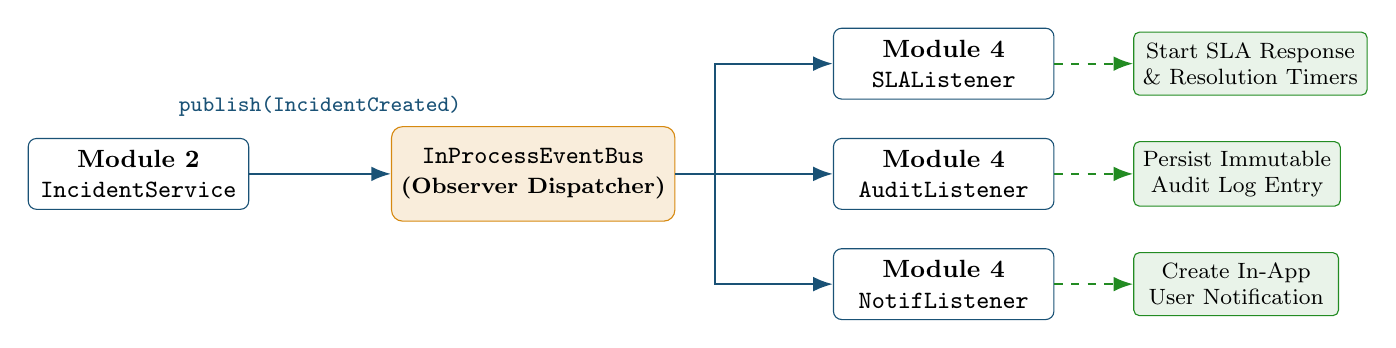
\begin{tikzpicture}[
    node distance=1.5cm,
    box/.style={rectangle, draw=primaryblue, fill=white, rounded corners=3pt, minimum width=2.8cm, minimum height=0.9cm, font=\small, align=center},
    busbox/.style={rectangle, draw=warningamber, fill=warningamber!15, rounded corners=4pt, minimum width=3.2cm, minimum height=1.2cm, font=\small\bfseries, align=center},
    actionbox/.style={rectangle, draw=forestgreen, fill=forestgreen!10, rounded corners=2pt, minimum width=2.6cm, minimum height=0.8cm, font=\footnotesize, align=center},
    arrow/.style={-{Latex[length=2.5mm]}, thick, primaryblue}
]

\node[box] (m2) {\textbf{Module 2}\\\texttt{IncidentService}};
\node[busbox, right=1.8cm of m2] (bus) {\texttt{InProcessEventBus}\\\footnotesize (Observer Dispatcher)};

\node[box, right=2.0cm of bus, yshift=1.4cm] (l1) {\textbf{Module 4}\\\texttt{SLAListener}};
\node[box, right=2.0cm of bus, yshift=0.0cm] (l2) {\textbf{Module 4}\\\texttt{AuditListener}};
\node[box, right=2.0cm of bus, yshift=-1.4cm] (l3) {\textbf{Module 4}\\\texttt{NotifListener}};

\node[actionbox, right=1.0cm of l1] (a1) {Start SLA Response\\\& Resolution Timers};
\node[actionbox, right=1.0cm of l2] (a2) {Persist Immutable\\Audit Log Entry};
\node[actionbox, right=1.0cm of l3] (a3) {Create In-App\\User Notification};

\draw[arrow] (m2) -- node[above, yshift=0.6cm, font=\footnotesize] {\texttt{publish(IncidentCreated)}} (bus);
\draw[arrow] (bus.east) -- ++(0.5,0) |- (l1.west);
\draw[arrow] (bus.east) -- ++(0.5,0) -- (l2.west);
\draw[arrow] (bus.east) -- ++(0.5,0) |- (l3.west);

\draw[arrow, dashed, forestgreen] (l1) -- (a1);
\draw[arrow, dashed, forestgreen] (l2) -- (a2);
\draw[arrow, dashed, forestgreen] (l3) -- (a3);

\end{tikzpicture}
\caption{Event-Driven Cross-Module Decoupling Architecture}
\label{fig:event_lifecycle}
\end{figure}

\section{Dependency Injection and Transaction Lifecycle}
\label{sec:arch_di}
FastAPI's dependency injection framework (\texttt{Depends}) enforces the \textbf{Dependency Inversion Principle} across all API endpoints:
\begin{itemize}
    \item Database sessions are managed per HTTP request via an asynchronous generator yielding an \texttt{AsyncSession}. Upon request completion, the session is committed or rolled back automatically.
    \item Endpoints declare dependencies on abstract interfaces. The injection container resolves these to concrete SQLAlchemy implementations within the per-request transaction context.
    \item In automated tests, \texttt{app.dependency\_overrides} seamlessly injects test doubles without modifying production codebase files.
\end{itemize}


\chapter{Module-Wise Technical Implementation}
\label{ch:modules}

\section{Module 1: Identity, Platform \& Administration}
\label{sec:module_m1}
\textbf{Owning Author:} Anay Goenka

Module 1 establishes the enterprise identity plane, credential security, role-based authorization rules, and centralized configuration registries utilized throughout the I-ITSM ecosystem.

\subsection{Domain Entities and Persistence Models}
M1 operates three primary database tables:
\begin{itemize}
    \item \texttt{UserModel} (\texttt{users} table): Represents system user identities. It records \texttt{id} (UUID primary key), \texttt{username} (unique string), \texttt{email} (unique string), \texttt{full\_name}, \texttt{password\_hash}, \texttt{role} (\texttt{EMPLOYEE}, \texttt{TECHNICIAN}, \texttt{ADMIN}), \texttt{is\_active} (boolean), and audit timestamps.
    \item \texttt{ServiceModel} (\texttt{services} table): Captures enterprise IT services. It records \texttt{id}, \texttt{name} (unique string), \texttt{description}, \texttt{business\_criticality} (integer scale from $1$ to $5$), \texttt{is\_active}, and timestamps.
    \item \texttt{CategoryModel} (\texttt{incident\_categories} table): Defines allowed ticket categories. It records \texttt{id}, \texttt{category} (unique string, e.g., \texttt{DATABASE}, \texttt{NETWORK}), \texttt{description}, \texttt{required\_skill} (string mapping to M3 competencies), and \texttt{is\_active}.
\end{itemize}

\subsection{Authentication and Cryptography}
User credentials are protected using salted Blowfish password hashing via the \texttt{bcrypt} library with a computational work factor of 12. Upon successful authentication against \texttt{POST /api/v1/auth/login}, the server generates a signed JSON Web Token (JWT) adhering to RFC 7519 standards. 

The JWT payload encodes the user's primary key in the subject claim (\texttt{sub}) and the assigned enterprise role in the \texttt{role} claim:
\begin{lstlisting}[language=json, caption={JWT Token Claims Payload}]
{
  "sub": "550e8400-e29b-41d4-a716-446655440000",
  "role": "TECHNICIAN",
  "exp": 1732245600
}
\end{lstlisting}

\subsection{Role-Based Access Control Guards}
FastAPI dependency injectors enforce declarative access control on API routes:
\begin{itemize}
    \item \texttt{get\_current\_user\_id}: Decodes the bearer token from the \texttt{Authorization} HTTP header, verifies the cryptographic signature, checks expiration, and retrieves the calling user's UUID.
    \item \texttt{require\_role(allowed\_roles)}: Evaluates the authenticated user's role against required permissions, returning HTTP 403 Forbidden if the user lacks authorization.
\end{itemize}

\subsection{User Provisioning Hook for Technicians}
When an administrator creates a user account with the \texttt{TECHNICIAN} role via \texttt{POST /api/v1/users}, M1 invokes a cross-module provisioning hook into M3's \texttt{TechnicianProfileService}. This automatically initializes an operational technician record with default availability (\texttt{AVAILABLE}), experience, and capacity limits, ensuring the technician can immediately participate in ticket assignment.

\subsection{Executive KPI Reporting}
The \texttt{/reports/summary} endpoint computes platform-wide operational KPIs by aggregating data across M1, M2, and M4, including active vs. resolved ticket counts, average MTTR, SLA compliance rates, and technician capacity utilization.

---

\section{Module 2: Incident Management \& Lifecycle Engine}
\label{sec:module_m2}
\textbf{Owning Author:} Anshul Naik

Module 2 governs the core business aggregate of the platform: the incident ticket, its progression state machine, collaboration notes, duplicate suppression, and audit-compliant archiving.

\subsection{Incident Aggregate and Database Models}
M2 manages two core persistence entities:
{\small\raggedright
\begin{itemize}
    \item \texttt{IncidentModel} (\texttt{incidents} table): Represents the canonical incident record. Fields include \texttt{id} (UUID primary key), \texttt{incident\_code} (unique \texttt{INC-xxxxxxxx}), \texttt{reporter\_id}, \texttt{service\_id}, \texttt{category}, \texttt{required\_skill}, \texttt{description}, \texttt{impact} ($1$--$5$), \texttt{urgency} ($1$--$5$), \texttt{business\_criticality} ($1$--$5$), \texttt{priority} ($P1$--$P4$), \texttt{status}, \texttt{assigned\_technician\_id}, \texttt{resolution\_details}, archiving columns (\texttt{is\_archived}, \texttt{archived\_at}, \texttt{archived\_by}),\linebreak and merging columns (\texttt{merged\_into\_incident\_id}, \texttt{merged\_at}, \texttt{merged\_by}).
    \item \texttt{IncidentCommentModel} (\texttt{incident\_comments} table): Captures timestamped collaboration notes and technical logs appended by stakeholders.
\end{itemize}
}

\subsection{Lifecycle State Machine}
The incident entity enforces a strict forward-progressing finite state machine:
\begin{equation}
\begin{aligned}
    \texttt{NEW} &\longrightarrow \texttt{CLASSIFIED} \longrightarrow \texttt{ASSIGNED} \longrightarrow \texttt{ACKNOWLEDGED} \\
    &\longrightarrow \texttt{IN\_PROGRESS} \longrightarrow \texttt{RESOLVED} \longrightarrow \texttt{VERIFIED} \longrightarrow \texttt{CLOSED}
\end{aligned}
\end{equation}

The state machine strictly enforces business invariants:
\begin{itemize}
    \item Backward transitions to previously satisfied lifecycle states are prohibited.
    \item Transitioning an incident to \texttt{RESOLVED} requires non-empty \texttt{resolution\_details}.
    \item Setting status to \texttt{CLOSED} or \texttt{ARCHIVED} is restricted to administrators and reporting users upon resolution verification.
\end{itemize}

\subsection{Duplicate Detection and Ticket Merging}
To prevent duplicate ticket proliferation, M2 includes the \texttt{DuplicateDetector} service. When evaluated, the detector tokenizes incident descriptions into character trigrams and computes the Dice similarity coefficient against active open tickets in the same category. Potential duplicates ($\text{similarity} \ge 0.65$) are surfaced to administrators. 

Upon administrative merge confirmation via \texttt{POST /api/v1/incidents/{id}/merge}, the secondary ticket is closed, its \texttt{merged\_into\_incident\_id} is set to the primary ticket, and cross-reference audit records are persisted.

\subsection{Soft-Archiving for Compliance}
To comply with enterprise data retention standards while maintaining responsive operational queues, M2 implements soft-archiving via \texttt{PATCH /api/v1/incidents/{id}/archive}. Soft-archived incidents are flagged as \texttt{is\_archived = true}, hidden from primary operational views, and queryable in a dedicated read-only historical archive.

---

\section{Module 3: Technician Management \& Assignment Engine}
\label{sec:module_m3}
\textbf{Owning Author:} Krish Jain

Module 3 maintains operational technician profiles, technical competency inventories, real-time workload metrics, deterministic assignment strategies, and AI-assisted candidate recommendation algorithms.

\subsection{Technician Domain Aggregate and Skills Matrix}
M3 manages two relational entities:
\begin{itemize}
    \item \texttt{TechnicianModel} (\texttt{technicians} table): Maintained in a strict 1:1 foreign key relationship with M1 \texttt{users.id}. It tracks \texttt{availability} (\texttt{AVAILABLE}, \texttt{BUSY}, \texttt{OFFLINE}, \texttt{ON\_LEAVE}), \texttt{experience\_years} ($\ge 0$), and \texttt{max\_capacity} ($\ge 1$).
    \item \texttt{TechnicianSkillModel} (\texttt{technician\_skills} table): Tracks technical proficiencies on a normalized 1 to 5 integer scale ($1$ = Novice, $5$ = Expert), associated with the technician profile with cascade deletion rules.
\end{itemize}

\subsection{Two-Phase Role Promotion and Operational Profile Lifecycle}
\label{sec:m3_two_phase_profile}
A critical architectural principle of I-ITSM is the strict separation between authentication identity (managed by M1 in the \texttt{users} table) and operational support capability (managed by M3 in the \texttt{technicians} and \texttt{technician\_skills} tables). In real-world enterprise environments, staff members are frequently promoted to technical support roles without requiring the re-creation of their corporate user identities.

To support this real-world operational requirement, M3 implements a two-phase onboarding workflow:
\begin{enumerate}
    \item \textbf{Phase 1: User Role Promotion:} An administrator updates an existing user's role to \texttt{TECHNICIAN} via \texttt{PATCH /api/v1/users/\{id\}}. The database immediately reflects the new role, but no operational profile exists yet.
    \item \textbf{Phase 2: Operational Roster Visibility and Profile Configuration:} The technician listing endpoint (\texttt{GET /api/v1/technicians}) performs an outer join between users with role \texttt{TECHNICIAN} and the \texttt{technicians} table. Newly promoted users appear in the roster with a distinct status badge: \textbf{Profile Not Configured} (\texttt{hasProfile = false}). Administrators can then open the profile creation modal to specify professional experience, maximum concurrent incident capacity, operational availability, and domain skills with $1$ to $5$ proficiency ratings.
\end{enumerate}
This ensures that promoted users are immediately identifiable, cannot be assigned incidents until their skills and capacity bounds are configured, and never require redundant account creation.

\subsection{Strategy Pattern for Algorithmic Assignment}
Technician assignment is architected around the Strategy Pattern:
\begin{itemize}
    \item \texttt{SkillBasedAssignmentStrategy}: Filters for available technicians with capacity headroom, scores candidates based on proficiency in the required skill ($20\times$) and experience bonus ($2\times$), and sorts candidates with deterministic tie-breaking.
    \item \texttt{LeastLoadedAssignmentStrategy}: Filters for available candidates and sorts in ascending order of active incident workload, prioritizing technicians with the highest remaining capacity headroom.
\end{itemize}

\subsection{Compare-and-Swap (CAS) Concurrency Protection}
To prevent technician over-allocation under concurrent assignment requests, \texttt{TechnicianAssignmentService} performs an optimistic Compare-and-Swap (CAS) capacity verification. Before persisting an assignment, the service re-queries the technician's active assigned incident count. If the count has reached \texttt{max\_capacity} due to an interleaved request, the transaction is rejected with HTTP 409 Conflict, preserving capacity invariants.

\subsection{Smart Recommendation Service and LLM Fallback}
The \texttt{SmartTechnicianRecommendationService} combines deterministic ranking with natural language reasoning via the \texttt{LLMProvider} adapter. The service constructs an anonymized prompt containing incident criteria and candidate proficiencies, querying the model for explanatory justification. If the external LLM is offline or exceeds a 2000\,ms timeout, the service seamlessly falls back to pure deterministic scoring, ensuring zero operational downtime.

---

\section{Module 4: SLA Tracking, Audit Logging \& Notifications}
\label{sec:module_m4}
\textbf{Owning Author:} Anirudh Yendalur

Module 4 provides automated SLA compliance governance, proactive warning detection, real-time user notification routing, and immutable audit logging.

\subsection{SLA Policy and Live Tracking Models}
M4 manages four relational entities:
\begin{itemize}
    \item \texttt{SLAPolicyModel} (\texttt{sla\_policies} table): Defines target response and resolution durations in hours for each priority tier ($P1$ through $P4$).
    \item \texttt{IncidentSLATrackingModel} (\texttt{incident\_sla\_tracking} table): Records live timing metrics for each incident, including \texttt{response\_due\_at}, \texttt{resolution\_due\_at}, \texttt{response\_breached}, \texttt{resolution\_breached}, \texttt{warning\_sent}, and operational status (\texttt{RUNNING}, \texttt{MET}, \texttt{BREACHED}, \texttt{WARNING}, \texttt{PAUSED}).
    \item \texttt{NotificationModel} (\texttt{notifications} table): Stores recipient alerts with notification type, title, message text, read status, and delivery timestamps.
    \item \texttt{AuditLogModel} (\texttt{audit\_logs} table): An immutable, append-only ledger capturing all system mutations with actor ID, action name, event type, previous state, new state, and contextual details.
\end{itemize}

\subsection{Asynchronous 60-Second Background SLA Monitor}
SLA compliance is continuously evaluated by the \texttt{SLAMonitorTask}, an asynchronous background worker initialized during FastAPI application startup:
\begin{enumerate}
    \item Every 60 seconds, the monitor queries the database for all active SLA tracking records in \texttt{RUNNING} or \texttt{WARNING} status.
    \item For each active record, it computes elapsed durations against target deadlines.
    \item \textbf{80\% Warning Threshold:} If elapsed time reaches or exceeds 80\% of the response or resolution target and \texttt{warning\_sent} is false, the monitor sets \texttt{warning\_sent = true}, transitions tracking status to \texttt{WARNING}, and dispatches an \texttt{SLAWarningEvent}.
    \item \textbf{Breach Threshold:} If elapsed time exceeds 100\% of the target duration, the monitor marks the respective breach flag (\texttt{response\_breached} or \texttt{resolution\_breached}), transitions status to \texttt{BREACHED}, and dispatches an \texttt{SLABreachedEvent}.
\end{enumerate}

\subsection{Notification Delivery and Real-Time Polling}
Notifications are routed to user inboxes upon domain event triggers. The frontend polls \texttt{GET /api/v1/notifications/unread/count} at 15-second intervals to maintain an updated notification badge. Users can view notifications, mark individual items as read, or invoke \texttt{PATCH /api/v1/notifications/read-all}.

\subsection{Event-Driven Listeners}
Module 4 registers three primary event observers on the \texttt{InProcessEventBus}:
\begin{itemize}
    \item \texttt{SLALifecycleEventListener}: Listens for \texttt{IncidentCreatedEvent} to initialize timers, \texttt{IncidentAssignedEvent} to record response timestamps, and \texttt{IncidentStatusChangedEvent} to evaluate resolution completion.
    \item \texttt{AuditEventListener}: Listens for all domain events, serializing actors, previous values, and new values into the append-only \texttt{audit\_logs} table.
    \item \texttt{NotificationEventListener}: Formats user-facing alert messages and persists them into the \texttt{notifications} table for affected stakeholders.
\end{itemize}


\chapter{Database Design \& Data Integrity}
\label{ch:database}

\section{Relational Schema Architecture}
\label{sec:db_architecture}
The persistence architecture of I-ITSM is built upon PostgreSQL 16+, utilizing a normalized relational design across eleven specialized tables. The database schema enforces strict referential integrity, domain constraint checks, and composite performance indexes.

Figure~\ref{fig:database_erd} presents the complete Entity-Relationship Diagram (ERD) capturing all tables and their foreign key relationships.

\begin{figure}[H]
\centering
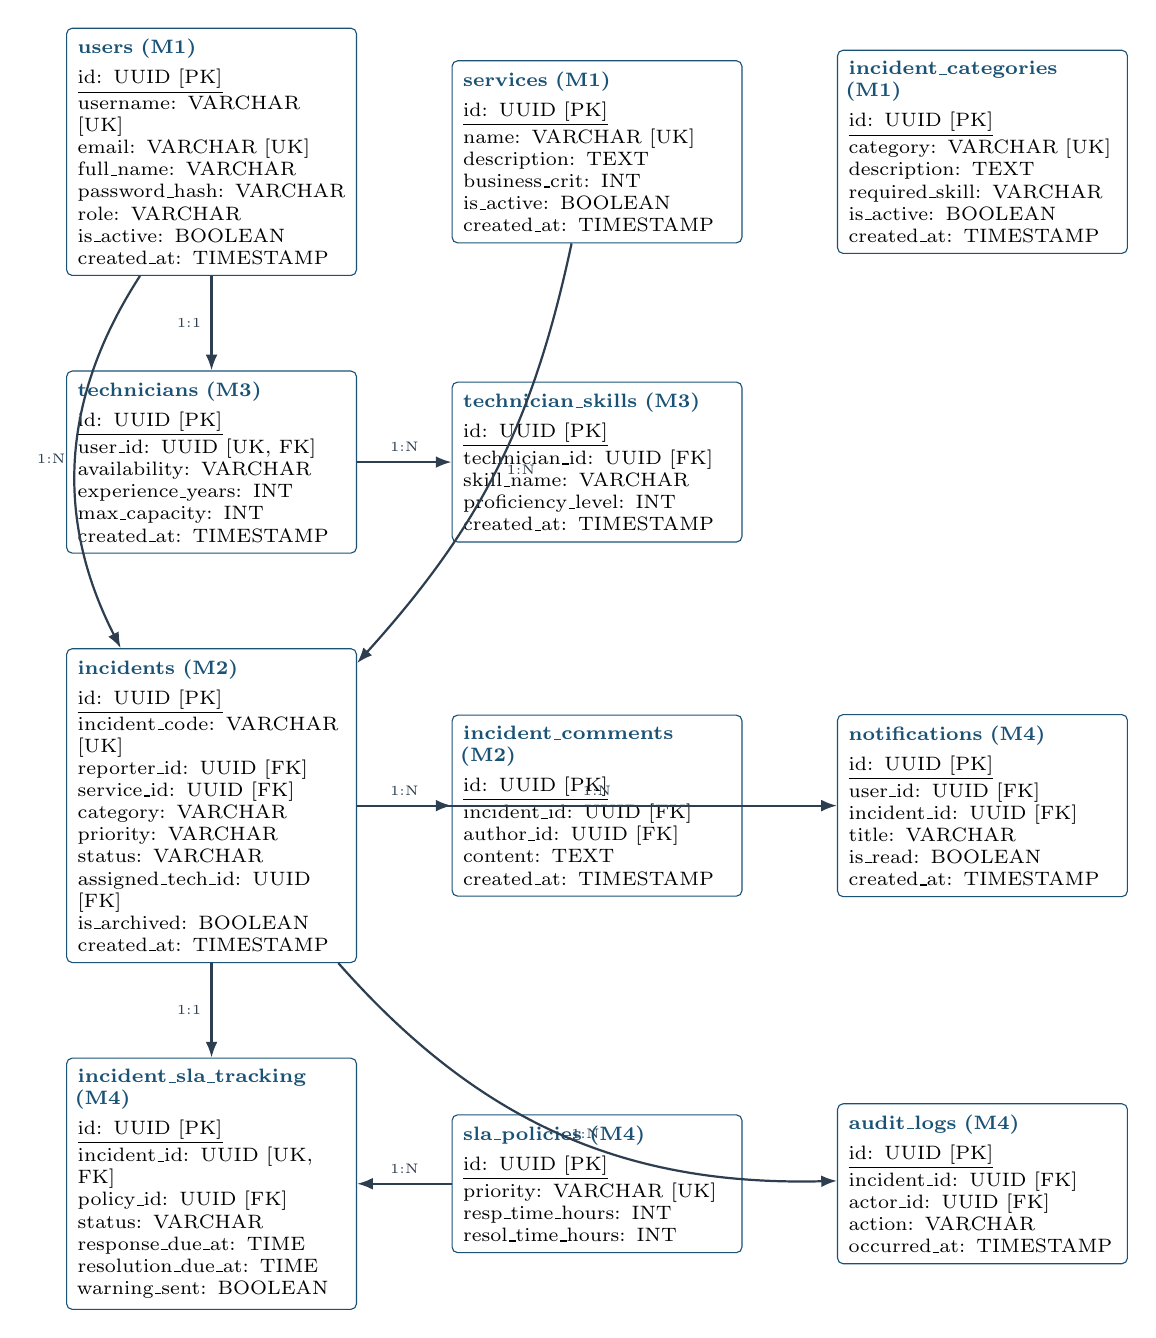
\begin{tikzpicture}[
    entity/.style={rectangle, draw=primaryblue, fill=white, rounded corners=2pt, text width=3.4cm, font=\scriptsize, inner sep=4pt},
    header/.style={fill=primaryblue!15, font=\scriptsize\bfseries, align=center},
    rel/.style={-{Latex[length=2mm]}, thick, darkslate}
]

% Row 1: Users, Services, Categories
\node[entity] (users) {
    \textbf{\textcolor{primaryblue}{users (M1)}}\\[0.1cm]
    \underline{id: UUID [PK]}\\
    username: VARCHAR [UK]\\
    email: VARCHAR [UK]\\
    full\_name: VARCHAR\\
    password\_hash: VARCHAR\\
    role: VARCHAR\\
    is\_active: BOOLEAN\\
    created\_at: TIMESTAMP
};

\node[entity, right=1.2cm of users] (services) {
    \textbf{\textcolor{primaryblue}{services (M1)}}\\[0.1cm]
    \underline{id: UUID [PK]}\\
    name: VARCHAR [UK]\\
    description: TEXT\\
    business\_crit: INT\\
    is\_active: BOOLEAN\\
    created\_at: TIMESTAMP
};

\node[entity, right=1.2cm of services] (categories) {
    \textbf{\textcolor{primaryblue}{incident\_categories (M1)}}\\[0.1cm]
    \underline{id: UUID [PK]}\\
    category: VARCHAR [UK]\\
    description: TEXT\\
    required\_skill: VARCHAR\\
    is\_active: BOOLEAN\\
    created\_at: TIMESTAMP
};

% Row 2: Technicians, Skills
\node[entity, below=1.2cm of users] (techs) {
    \textbf{\textcolor{primaryblue}{technicians (M3)}}\\[0.1cm]
    \underline{id: UUID [PK]}\\
    user\_id: UUID [UK, FK]\\
    availability: VARCHAR\\
    experience\_years: INT\\
    max\_capacity: INT\\
    created\_at: TIMESTAMP
};

\node[entity, right=1.2cm of techs] (skills) {
    \textbf{\textcolor{primaryblue}{technician\_skills (M3)}}\\[0.1cm]
    \underline{id: UUID [PK]}\\
    technician\_id: UUID [FK]\\
    skill\_name: VARCHAR\\
    proficiency\_level: INT\\
    created\_at: TIMESTAMP
};

% Row 3: Incidents, Comments
\node[entity, below=1.2cm of techs] (incidents) {
    \textbf{\textcolor{primaryblue}{incidents (M2)}}\\[0.1cm]
    \underline{id: UUID [PK]}\\
    incident\_code: VARCHAR [UK]\\
    reporter\_id: UUID [FK]\\
    service\_id: UUID [FK]\\
    category: VARCHAR\\
    priority: VARCHAR\\
    status: VARCHAR\\
    assigned\_tech\_id: UUID [FK]\\
    is\_archived: BOOLEAN\\
    created\_at: TIMESTAMP
};

\node[entity, right=1.2cm of incidents] (comments) {
    \textbf{\textcolor{primaryblue}{incident\_comments (M2)}}\\[0.1cm]
    \underline{id: UUID [PK]}\\
    incident\_id: UUID [FK]\\
    author\_id: UUID [FK]\\
    content: TEXT\\
    created\_at: TIMESTAMP
};

% Row 4: SLA, Audit, Notifications
\node[entity, below=1.2cm of incidents] (sla_track) {
    \textbf{\textcolor{primaryblue}{incident\_sla\_tracking (M4)}}\\[0.1cm]
    \underline{id: UUID [PK]}\\
    incident\_id: UUID [UK, FK]\\
    policy\_id: UUID [FK]\\
    status: VARCHAR\\
    response\_due\_at: TIME\\
    resolution\_due\_at: TIME\\
    warning\_sent: BOOLEAN
};

\node[entity, right=1.2cm of sla_track] (sla_policy) {
    \textbf{\textcolor{primaryblue}{sla\_policies (M4)}}\\[0.1cm]
    \underline{id: UUID [PK]}\\
    priority: VARCHAR [UK]\\
    resp\_time\_hours: INT\\
    resol\_time\_hours: INT
};

\node[entity, right=1.2cm of sla_policy] (audit) {
    \textbf{\textcolor{primaryblue}{audit\_logs (M4)}}\\[0.1cm]
    \underline{id: UUID [PK]}\\
    incident\_id: UUID [FK]\\
    actor\_id: UUID [FK]\\
    action: VARCHAR\\
    occurred\_at: TIMESTAMP
};

\node[entity, right=1.2cm of comments] (notif) {
    \textbf{\textcolor{primaryblue}{notifications (M4)}}\\[0.1cm]
    \underline{id: UUID [PK]}\\
    user\_id: UUID [FK]\\
    incident\_id: UUID [FK]\\
    title: VARCHAR\\
    is\_read: BOOLEAN\\
    created\_at: TIMESTAMP
};

% Relationships
\draw[rel] (users) -- node[left, font=\tiny] {1:1} (techs);
\draw[rel] (techs) -- node[above, font=\tiny] {1:N} (skills);
\draw[rel] (users) to[bend right=30] node[left, font=\tiny] {1:N} (incidents);
\draw[rel] (services) to[bend left=15] node[right, font=\tiny] {1:N} (incidents);
\draw[rel] (incidents) -- node[above, font=\tiny] {1:N} (comments);
\draw[rel] (incidents) -- node[left, font=\tiny] {1:1} (sla_track);
\draw[rel] (sla_policy) -- node[above, font=\tiny] {1:N} (sla_track);
\draw[rel] (incidents) to[bend right=25] node[right, font=\tiny] {1:N} (audit);
\draw[rel] (incidents) -- node[above, font=\tiny] {1:N} (notif);

\end{tikzpicture}
\caption{Entity-Relationship Diagram of the I-ITSM Relational Schema}
\label{fig:database_erd}
\end{figure}

\section{Detailed Table Catalog and Constraints}
\label{sec:db_tables}

\begin{table}[H]
\centering
\small
\caption{Database Schema Table Inventory and Module Ownership}
\label{tab:db_inventory}
\begin{tabular}{p{3.2cm}p{1.8cm}p{3.8cm}p{6.0cm}}
\toprule
\textbf{Table Name} & \textbf{Module} & \textbf{Primary Constraints} & \textbf{Functional Purpose} \\
\midrule
\texttt{users} & M1 & PK: \texttt{id}, UK: \texttt{username}, \texttt{email} & Enterprise user accounts, salted password hashes, and system roles. \\
\addlinespace
\texttt{services} & M1 & PK: \texttt{id}, UK: \texttt{name} & IT service catalogue entries with business criticality ratings ($1$--$5$). \\
\addlinespace
\texttt{incident\_categories} & M1 & PK: \texttt{id}, UK: \texttt{category} & Incident categories mapped to required technical skills. \\
\addlinespace
\texttt{technicians} & M3 & PK: \texttt{id}, UK/FK: \texttt{user\_id} & Operational technician profiles, availability states, experience, and capacity. \\
\addlinespace
\texttt{technician\_skills} & M3 & PK: \texttt{id}, FK: \texttt{technician\_id} (Cascade) & Technical skills and numeric proficiency levels ($1$--$5$) per technician. \\
\addlinespace
\texttt{incidents} & M2 & PK: \texttt{id}, UK: \texttt{incident\_code} & Core incident records, calculated priorities ($P1$--$P4$), status, and assignment. \\
\addlinespace
\texttt{incident\_comments} & M2 & PK: \texttt{id}, FK: \texttt{incident\_id} (Cascade) & Chronological discussion notes and collaboration logs. \\
\addlinespace
\texttt{sla\_policies} & M4 & PK: \texttt{id}, UK: \texttt{priority} & Standard target response and resolution durations for $P1$--$P4$. \\
\addlinespace
\texttt{incident\_sla\_tracking} & M4 & PK: \texttt{id}, UK: \texttt{incident\_id} & Real-time tracking records capturing target deadlines, warnings, and breaches. \\
\addlinespace
\texttt{audit\_logs} & M4 & PK: \texttt{id}, FK: \texttt{incident\_id}, \texttt{actor\_id} & Immutable append-only audit trail capturing system-wide operational mutations. \\
\addlinespace
\texttt{notifications} & M4 & PK: \texttt{id}, FK: \texttt{user\_id} & User alert delivery inbox with read/unread flags and timestamps. \\
\bottomrule
\end{tabular}
\end{table}

\section{Indexing Strategy and Performance Optimization}
\label{sec:db_indexing}
To ensure that queries execute in $< 50$\,ms even under high data volume, specific indexes were established:
\begin{itemize}
    \item \texttt{ix\_incidents\_status\_priority}: Composite B-Tree index on \texttt{incidents(status, priority)} accelerating operational queue filtering by urgency and lifecycle state.
    \item \texttt{ix\_incidents\_reporter\_created}: Composite index on \texttt{incidents(reporter\_id, created\_at DESC)} optimizing employee dashboard timeline queries.
    \item \texttt{ix\_incidents\_assigned\_status}: Composite index on \texttt{incidents(assigned\_technician\_id, status)} optimizing technician active workload calculation.
    \item \texttt{ix\_incidents\_is\_archived}: B-Tree index separating active operational tickets from soft-archived compliance records.
    \item \texttt{ix\_technician\_skills\_skill\_name}: Index on \texttt{technician\_skills(skill\_name)} accelerating candidate filtering during recommendation runs.
    \item \texttt{ix\_notifications\_user\_read}: Composite index on \texttt{notifications(user\_id, is\_read)} optimizing unread badge counter polling (\texttt{/notifications/unread/count}).
    \item \texttt{ix\_audit\_logs\_incident\_occurred}: Index on \texttt{audit\_logs(incident\_id, occurred\_at DESC)} optimizing chronological audit trail queries.
\end{itemize}

\section{Alembic Database Migration History}
\label{sec:db_migrations}
Database evolution is strictly version-controlled through six sequential Alembic revisions stored in \texttt{backend/migrations/versions/}:
\begin{enumerate}
    \item \textbf{Revision 001 (\texttt{001\_initial\_technician\_schema.py}):} Creates the initial operational tables \texttt{technicians} and \texttt{technician\_skills}.
    \item \textbf{Revision 002 (\texttt{002\_create\_users.py}):} Provisions the primary \texttt{users} table with authentication fields, roles, and uniqueness constraints.
    \item \textbf{Revision 003 (\texttt{003\_services\_and\_categories.py}):} Establishes enterprise configuration tables \texttt{services} and \texttt{incident\_categories}.
    \item \textbf{Revision 004 (\texttt{004\_incidents\_and\_comments.py}):} Introduces core ticketing tables \texttt{incidents} and \texttt{incident\_comments} with foreign keys and status enums.
    \item \textbf{Revision 005 (\texttt{005\_sla\_audit\_notifications.py}):} Provisions governance tables \texttt{sla\_policies}, \texttt{incident\_sla\_tracking}, \texttt{audit\_logs}, and \texttt{notifications}.
    \item \textbf{Revision 006 (\texttt{006\_incident\_archive\_merge.py}):} Extends \texttt{incidents} with soft-archiving columns (\texttt{is\_archived}, \texttt{archived\_at}, \texttt{archived\_by}) and merging columns (\texttt{merged\_into\_incident\_id}, \texttt{merged\_at}, \texttt{merged\_by}).
\end{enumerate}


\chapter{Algorithms \& Business Logic}
\label{ch:algorithms}

\section{Priority Scoring Matrix Algorithm}
\label{sec:algo_priority}
To prevent subjective human classification bias, incident priority is evaluated mathematically using a multi-factor linear scoring matrix implemented in \texttt{PriorityCalculator}.

\subsection{Mathematical Formulation}
Let $I \in [1, 5]$ denote the reported incident impact, $U \in [1, 5]$ denote urgency, and $C \in [1, 5]$ denote the business criticality of the affected IT service. The continuous composite score $S \in [1.0, 5.0]$ is computed as:
\begin{equation}
S = (0.4 \times I) + (0.4 \times U) + (0.2 \times C)
\end{equation}

The continuous score $S$ is deterministically mapped to standardized ITIL priority levels via threshold bucketing:
\begin{equation}
\text{Priority}(S) = 
\begin{cases}
P1 \text{ (Critical)}, & \text{if } S \ge 4.0 \\
P2 \text{ (High)}, & \text{if } 3.0 \le S < 4.0 \\
P3 \text{ (Medium)}, & \text{if } 2.0 \le S < 3.0 \\
P4 \text{ (Low)}, & \text{if } S < 2.0
\end{cases}
\end{equation}

\subsection{Algorithm Pseudocode}
Listing~\ref{lst:algo_priority} details the priority calculation routine.

\begin{lstlisting}[language=Python, caption={Priority Calculation Matrix Routine}, label={lst:algo_priority}]
def calculate_priority(impact: int, urgency: int, business_criticality: int) -> str:
    # Validate input bounds
    assert 1 <= impact <= 5 and 1 <= urgency <= 5 and 1 <= business_criticality <= 5
    
    # Compute weighted composite score
    score = (impact * 0.4) + (urgency * 0.4) + (business_criticality * 0.2)
    
    # Threshold bucketing
    if score >= 4.0:
        return "P1"
    elif score >= 3.0:
        return "P2"
    elif score >= 2.0:
        return "P3"
    else:
        return "P4"
\end{lstlisting}

---

\section{Duplicate Incident Detection Algorithm}
\label{sec:algo_duplicate}
To prevent duplicate ticket processing, the \texttt{DuplicateDetector} computes textual similarity between an incoming incident description and open tickets within the same category.

\subsection{Trigram Tokenization and Similarity Formulation}
Given text $T$, let $\text{Tri}(T)$ be the multiset of 3-character substrings (trigrams) extracted after lowercasing and punctuation stripping. For candidate descriptions $A$ and $B$, the Dice similarity coefficient $D(A, B) \in [0.0, 1.0]$ is:
\begin{equation}
D(A, B) = \frac{2 \times |\text{Tri}(A) \cap \text{Tri}(B)|}{|\text{Tri}(A)| + |\text{Tri}(B)|}
\end{equation}

If $D(A, B) \ge 0.65$, ticket $B$ is classified as a potential duplicate of $A$.

\subsection{Algorithm Pseudocode}
Listing~\ref{lst:algo_duplicate} details the duplicate detection procedure.

\begin{lstlisting}[language=Python, caption={Duplicate Incident Detection via Trigram Overlap}, label={lst:algo_duplicate}]
def find_potential_duplicates(target_incident, open_incidents, threshold=0.65):
    target_trigrams = extract_trigrams(target_incident.description)
    duplicates = []
    
    for candidate in open_incidents:
        if candidate.id == target_incident.id:
            continue
        if candidate.category != target_incident.category:
            continue
            
        candidate_trigrams = extract_trigrams(candidate.description)
        intersection = len(target_trigrams & candidate_trigrams)
        total = len(target_trigrams) + len(candidate_trigrams)
        
        similarity = (2.0 * intersection) / total if total > 0 else 0.0
        
        if similarity >= threshold:
            duplicates.append((candidate, round(similarity, 4)))
            
    return sorted(duplicates, key=lambda x: x[1], reverse=True)
\end{lstlisting}

---

\section{Skill-Based Technician Assignment Strategy}
\label{sec:algo_skill_assign}
The \texttt{SkillBasedAssignmentStrategy} ranks candidates based on competency in the incident's required skill and professional experience.

\subsection{Scoring and Deterministic Ranking}
Let $T$ be an operational technician candidate. $T$ is eligible if:
\begin{equation}
\text{availability}(T) = \texttt{AVAILABLE} \quad \text{and} \quad \text{active\_incidents}(T) < \text{max\_capacity}(T)
\end{equation}

For eligible candidates, let $p \in [1, 5]$ be the technician's proficiency in the required skill (or $0$ if absent), and let $e \ge 0$ denote professional experience in years. The composite match score is:
\begin{equation}
\text{Score}(T) = (p \times 20) + (e \times 2)
\end{equation}

Candidates are sorted according to the tuple:
\begin{equation}
\text{SortKey}(T) = \left(-\text{Score}(T), \; \text{active\_incidents}(T), \; \text{user\_id}(T)\right)
\end{equation}
This prioritizes high competency, breaks ties in favor of lower workload, and breaks secondary ties deterministically using UUID string ordering.

---

\section{Least-Loaded Technician Assignment Strategy}
\label{sec:algo_least_loaded}
The \texttt{LeastLoadedAssignmentStrategy} balances queue volume across available staff. Eligible candidates are sorted using the key:
\begin{equation}
\text{SortKey}(T) = \left(\text{active\_incidents}(T), \; -e(T), \; \text{user\_id}(T)\right)
\end{equation}
This selects the technician with the lowest active incident count, breaking ties in favor of higher experience.

---

\section{Compare-and-Swap (CAS) Concurrency Protection}
\label{sec:algo_cas}
To prevent over-allocation when concurrent assignment requests target the same technician, \texttt{TechnicianAssignmentService} executes an optimistic Compare-and-Swap verification:

\begin{lstlisting}[language=Python, caption={Compare-and-Swap Capacity Protection Routine}, label={lst:algo_cas}]
async def assign_incident_atomic(session, incident_id, technician_id):
    async with session.begin():
        # Lock technician profile record for update
        tech = await get_technician_for_update(session, technician_id)
        if tech.availability != "AVAILABLE":
            raise ConflictException("Technician is not currently available.")
            
        current_workload = await count_active_incidents(session, technician_id)
        if current_workload >= tech.max_capacity:
            raise ConflictException("Technician has reached maximum capacity.")
            
        # Execute assignment update
        await update_incident_assignment(session, incident_id, technician_id)
        # Event is dispatched post-commit
\end{lstlisting}

---

\section{Periodic SLA Monitor Sweep Algorithm}
\label{sec:algo_sla_sweep}
The background \texttt{SLAMonitorTask} evaluates active tickets every 60 seconds:

\begin{lstlisting}[language=Python, caption={Periodic SLA Monitor Sweep Routine}, label={lst:algo_sla}]
async def execute_sla_sweep(session, event_bus):
    active_trackers = await get_active_sla_trackers(session)
    now = datetime.utcnow()
    
    for tracker in active_trackers:
        policy = await get_sla_policy(session, tracker.priority)
        target_resolution_hours = policy.resolution_time_hours
        elapsed_seconds = (now - tracker.started_at).total_seconds()
        target_seconds = target_resolution_hours * 3600
        
        # 80% Warning Evaluation
        if (elapsed_seconds >= 0.8 * target_seconds) and not tracker.warning_sent:
            tracker.warning_sent = True
            tracker.status = "WARNING"
            await event_bus.publish(SLAWarningEvent(tracker.incident_id))
            
        # 100% Breach Evaluation
        if (elapsed_seconds >= target_seconds) and not tracker.resolution_breached:
            tracker.resolution_breached = True
            tracker.status = "BREACHED"
            await event_bus.publish(SLABreachedEvent(tracker.incident_id))
            
    await session.commit()
\end{lstlisting}


\chapter{Backend Implementation Details}
\label{ch:backend}

\section{FastAPI Lifespan and Application Initialization}
\label{sec:backend_lifespan}
The backend service initializes via FastAPI's modern asynchronous \texttt{lifespan} context manager. During application startup, the lifespan routine:
\begin{enumerate}
    \item Initializes the SQLAlchemy \texttt{AsyncEngine} and validates database connectivity to PostgreSQL 16+.
    \item Subscribes domain event observers (\texttt{SLALifecycleEventListener}, \texttt{AuditEventListener}, \texttt{NotificationEventListener}) to the global \texttt{InProcessEventBus}.
    \item Spawns the background \texttt{SLAMonitorTask} daemon as an asynchronous coroutine running concurrently with incoming HTTP request processing.
\end{enumerate}

Upon shutdown, the lifespan routine cleanly cancels the background monitor task, commits pending transactions, and disposes of the connection pool.

\section{Complete REST API Route Reference}
\label{sec:backend_routes}
The I-ITSM backend exposes exactly 41 REST API endpoints under the \texttt{/api/v1} prefix, summarized in Table~\ref{tab:api_route_inventory}.

\begin{table}[H]
\centering
\scriptsize
\caption{Complete REST API Endpoint Inventory (41 Routes)}
\label{tab:api_route_inventory}
\begin{tabular}{p{1.2cm}p{5.5cm}p{2.5cm}p{5.0cm}}
\toprule
\textbf{Method} & \textbf{Endpoint Path} & \textbf{Authentication} & \textbf{Functional Purpose} \\
\midrule
\multicolumn{4}{l}{\textbf{Module 1: Authentication, Users, Platform \& Catalog}} \\
\midrule
\texttt{POST} & \texttt{/api/v1/auth/register} & Public & User registration (default \texttt{EMPLOYEE} role). \\
\texttt{POST} & \texttt{/api/v1/auth/login} & Public & User login; returns signed JWT access token. \\
\texttt{GET} & \texttt{/api/v1/auth/me} & Any Authenticated & Retrieves current logged-in user profile. \\
\texttt{GET} & \texttt{/api/v1/users} & Admin Only & Lists all registered system users. \\
\texttt{POST} & \texttt{/api/v1/users} & Admin Only & Creates new user; auto-provisions tech profile. \\
\texttt{GET} & \texttt{/api/v1/users/summary} & Admin Only & Returns user statistics by role and activity. \\
\texttt{GET} & \texttt{/api/v1/users/\{user\_id\}} & Admin Only & Retrieves details for a specific user. \\
\texttt{PATCH} & \texttt{/api/v1/users/\{user\_id\}} & Admin Only & Updates user full name, role, or active status. \\
\texttt{DELETE} & \texttt{/api/v1/users/\{user\_id\}} & Admin Only & Soft-deactivates user (prevents self-deactivation). \\
\texttt{GET} & \texttt{/api/v1/services} & Any Authenticated & Lists active IT service catalogue items. \\
\texttt{POST} & \texttt{/api/v1/services} & Admin Only & Adds service with business criticality ($1$--$5$). \\
\texttt{PATCH} & \texttt{/api/v1/services/\{id\}} & Admin Only & Updates service details or criticality rating. \\
\texttt{DELETE} & \texttt{/api/v1/services/\{id\}} & Admin Only & Deactivates service catalogue entry. \\
\texttt{GET} & \texttt{/api/v1/categories} & Any Authenticated & Lists incident categories and skill mappings. \\
\texttt{POST} & \texttt{/api/v1/categories} & Admin Only & Adds new category-to-skill mapping. \\
\texttt{PATCH} & \texttt{/api/v1/categories/\{id\}} & Admin Only & Updates category definition or skill mapping. \\
\texttt{DELETE} & \texttt{/api/v1/categories/\{id\}} & Admin Only & Deactivates incident category. \\
\texttt{GET} & \texttt{/api/v1/reports/summary} & Admin Only & Computes executive KPI summary across modules. \\
\midrule
\multicolumn{4}{l}{\textbf{Module 2: Incident Management \& Lifecycle}} \\
\midrule
\texttt{POST} & \texttt{/api/v1/incidents} & Employee / Admin & Creates incident; calculates priority ($P1$--$P4$). \\
\texttt{GET} & \texttt{/api/v1/incidents} & Any Authenticated & Lists incidents filtered by role and criteria. \\
\texttt{GET} & \texttt{/api/v1/incidents/archived} & Admin Only & Lists soft-archived historical incidents. \\
\texttt{GET} & \texttt{/api/v1/incidents/\{id\}} & Any Authenticated & Retrieves incident details with comment thread. \\
\texttt{PATCH} & \texttt{/api/v1/incidents/\{id\}} & Any Authenticated & Updates description/urgency; recomputes priority. \\
\texttt{PATCH} & \texttt{/api/v1/incidents/\{id\}/status} & Tech / Admin & Advances state machine (requires details on resolve). \\
\texttt{PATCH} & \texttt{/api/v1/incidents/\{id\}/archive} & Admin Only & Soft-archives closed ticket for compliance. \\
\texttt{POST} & \texttt{/api/v1/incidents/\{id\}/comments} & Any Authenticated & Appends collaboration comment note. \\
\texttt{GET} & \texttt{/api/v1/incidents/\{id\}/duplicates}& Admin Only & Computes trigram similarity duplicate candidates. \\
\texttt{POST} & \texttt{/api/v1/incidents/\{id\}/merge} & Admin Only & Merges duplicate ticket into primary incident. \\
\texttt{POST} & \texttt{/api/v1/incidents/\{id\}/assign} & Admin Only & Assigns technician with CAS capacity protection. \\
\midrule
\multicolumn{4}{l}{\textbf{Module 3: Technician Management \& Assignment Engine}} \\
\midrule
\texttt{GET} & \texttt{/api/v1/technicians} & Any Authenticated & Lists technicians with workloads and skills. \\
\texttt{GET} & \texttt{/api/v1/technicians/recommendations}& Admin Only & Algorithmic/LLM technician recommendation. \\
\texttt{GET} & \texttt{/api/v1/technicians/\{id\}} & Any Authenticated & Retrieves specific technician operational profile. \\
\texttt{PATCH} & \texttt{/api/v1/technicians/\{id\}} & Admin Only & Updates technician experience and capacity. \\
\texttt{PATCH} & \texttt{/api/v1/technicians/\{id\}/availability}& Tech / Admin & Updates availability (\texttt{AVAILABLE} $\leftrightarrow$ \texttt{BUSY}). \\
\texttt{GET} & \texttt{/api/v1/technicians/\{id\}/skills} & Any Authenticated & Retrieves technician skill competencies. \\
\texttt{POST} & \texttt{/api/v1/technicians/\{id\}/skills} & Tech / Admin & Adds or updates skill proficiency rating ($1$--$5$). \\
\texttt{DELETE} & \texttt{/api/v1/technicians/\{id\}/skills/\{s\}}& Tech / Admin & Removes skill from technician profile. \\
\midrule
\multicolumn{4}{l}{\textbf{Module 4: SLA Tracking, Audit Logging \& Notifications}} \\
\midrule
\texttt{GET} & \texttt{/api/v1/sla/policies} & Any Authenticated & Lists standard SLA target durations for $P1$--$P4$. \\
\texttt{POST} & \texttt{/api/v1/sla/policies} & Admin Only & Creates new SLA priority policy. \\
\texttt{PATCH} & \texttt{/api/v1/sla/policies/\{priority\}} & Admin Only & Updates response/resolution targets for a priority. \\
\texttt{GET} & \texttt{/api/v1/sla/summary} & Admin Only & Returns compliance rate and active warning counts. \\
\texttt{GET} & \texttt{/api/v1/sla/violations} & Admin Only & Lists breached and approaching-warning tickets. \\
\texttt{POST} & \texttt{/api/v1/sla/check} & Admin Only & Manually triggers on-demand SLA sweep cycle. \\
\texttt{GET} & \texttt{/api/v1/incidents/\{id\}/sla} & Any Authenticated & Retrieves live SLA tracking status for a ticket. \\
\texttt{GET} & \texttt{/api/v1/notifications} & Any Authenticated & Lists notifications for the authenticated user. \\
\texttt{GET} & \texttt{/api/v1/notifications/unread} & Any Authenticated & Lists unread notifications. \\
\texttt{GET} & \texttt{/api/v1/notifications/unread/count}& Any Authenticated & Lightweight unread count for badge polling. \\
\texttt{PATCH} & \texttt{/api/v1/notifications/\{id\}/read} & Any Authenticated & Marks individual notification as read. \\
\texttt{PATCH} & \texttt{/api/v1/notifications/read-all} & Any Authenticated & Marks all user notifications as read. \\
\texttt{GET} & \texttt{/api/v1/audit} & Admin Only & Queries system-wide audit logs with filters. \\
\texttt{GET} & \texttt{/api/v1/incidents/\{id\}/audit} & Any Authenticated & Chronological audit trail for specific incident. \\
\bottomrule
\end{tabular}
\end{table}

\section{Dependency Injection and Asynchronous Sessions}
\label{sec:backend_di}
FastAPI's dependency injection system governs all database transactions. The session provider yields an \texttt{AsyncSession} tied to the request lifecycle:
\begin{lstlisting}[language=Python, caption={Per-Request Async Database Session Provider}]
async def get_db_session() -> AsyncGenerator[AsyncSession, None]:
    async with AsyncSessionLocal() as session:
        try:
            yield session
            await session.commit()
        except Exception:
            await session.rollback()
            raise
        finally:
            await session.close()
\end{lstlisting}

\section{Pydantic v2 DTOs and Response Formatting}
\label{sec:backend_dto}
All API inputs and outputs are strictly typed via Pydantic v2 models. Input models enforce validation constraints (e.g., impact and urgency within $[1, 5]$). Output DTOs configure automatic camelCase serialization for seamless React integration:
\begin{lstlisting}[language=Python, caption={Pydantic DTO Configuration with CamelCase Aliasing}]
class BaseDTO(BaseModel):
    model_config = ConfigDict(
        from_attributes=True,
        populate_by_name=True,
        alias_generator=to_camel_case
    )
\end{lstlisting}

\section{Global Exception Handling and Error Envelope}
\label{sec:backend_errors}
The application registers global exception handlers ensuring consistent error responses across all failure modes:
\begin{lstlisting}[language=json, caption={Standardized JSON Error Envelope}]
{
  "detail": "Technician has reached maximum capacity of 5 active tickets."
}
\end{lstlisting}
This consistent structure guarantees that the frontend error parser can extract meaningful messages without handling heterogeneous payload shapes.


\chapter{Frontend Implementation Details}
\label{ch:frontend}

\section{React Single-Page Application Architecture}
\label{sec:frontend_arch}
The I-ITSM frontend is engineered as a modern Single-Page Application (SPA) utilizing React 18, Vite, and React Router DOM v6. The client architecture emphasizes modular component hierarchies, deterministic state management, responsive user feedback, and accessibility.

Figure~\ref{fig:frontend_component_tree} illustrates the top-level component architecture and routing layout.

\begin{figure}[H]
\centering
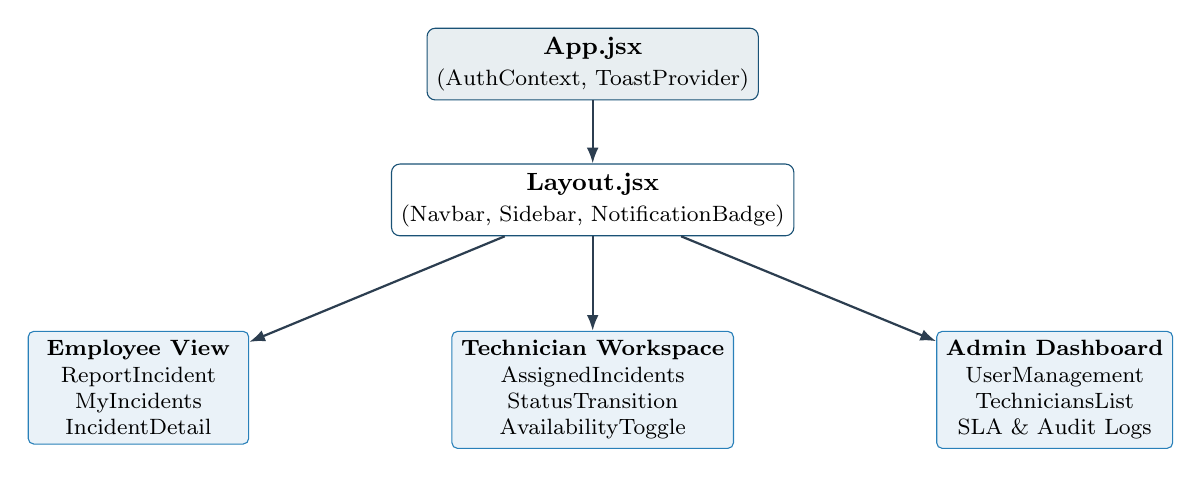
\begin{tikzpicture}[
    comp/.style={rectangle, draw=primaryblue, fill=white, rounded corners=3pt, minimum width=3.2cm, minimum height=0.8cm, font=\small, align=center},
    routecomp/.style={rectangle, draw=secondaryblue, fill=secondaryblue!10, rounded corners=2pt, minimum width=2.8cm, minimum height=0.7cm, font=\footnotesize, align=center},
    arrow/.style={-{Latex[length=2mm]}, thick, darkslate}
]

\node[comp, fill=primaryblue!10] (app) {\textbf{App.jsx}\\\footnotesize (AuthContext, ToastProvider)};
\node[comp, below=0.8cm of app] (layout) {\textbf{Layout.jsx}\\\footnotesize (Navbar, Sidebar, NotificationBadge)};

\node[routecomp, below left=1.2cm and 1.8cm of layout] (emp) {\textbf{Employee View}\\ReportIncident\\MyIncidents\\IncidentDetail};
\node[routecomp, below=1.2cm of layout] (tech) {\textbf{Technician Workspace}\\AssignedIncidents\\StatusTransition\\AvailabilityToggle};
\node[routecomp, below right=1.2cm and 1.8cm of layout] (adm) {\textbf{Admin Dashboard}\\UserManagement\\TechniciansList\\SLA \& Audit Logs};

\draw[arrow] (app) -- (layout);
\draw[arrow] (layout) -- (emp);
\draw[arrow] (layout) -- (tech);
\draw[arrow] (layout) -- (adm);

\end{tikzpicture}
\caption{Frontend Component Hierarchy and Role-Based Route Distribution}
\label{fig:frontend_component_tree}
\end{figure}

\section{Role-Based Navigation and View Access Control}
\label{sec:frontend_rbac}
The frontend enforces role-based navigation via the \texttt{ProtectedRoute} component, which inspects the authenticated user's role:
\begin{itemize}
    \item \textbf{Employee Portal:} Displays a streamlined interface containing ``Report Incident'' (with service and category pickers), ``My Reported Incidents'' timeline, and interactive discussion threads.
    \item \textbf{Technician Workspace:} Displays the technician's assigned ticket queue, visual SLA countdown indicators, forward status transition action buttons, and an instant operational availability toggle (\texttt{AVAILABLE} $\leftrightarrow$ \texttt{BUSY}).
    \item \textbf{Admin Management Console:} Provides full management capabilities, including ``User Management'' (with user search, role updates, and modal user provisioning), ``Manage Technicians'' (displaying technician usernames, workload metrics, and skills), ``Service \& Category Catalogs'', ``SLA Policies \& Violations'', and ``System Audit Trail''.
\end{itemize}

\section{Centralized Frontend Error Extraction Utility}
\label{sec:frontend_error_util}
A common flaw in REST client applications is the presentation of generic, opaque error messages (such as ``Request failed with status code 409''). To deliver a superior user experience, I-ITSM incorporates a centralized error-handling utility: \texttt{frontend/src/utils/errorHandler.js}.

The utility intercepts HTTP errors and executes a multi-stage extraction strategy:
\begin{lstlisting}[language=JavaScript, caption={Centralized Error Extraction Logic (`errorHandler.js`)}]
export function extractErrorMessage(error, fallback = "An unexpected error occurred.") {
  if (!error) return fallback;
  
  // 1. Direct Backend Error Response Detail
  if (error.response?.data?.detail) {
    const detail = error.response.data.detail;
    if (typeof detail === "string") return detail;
    if (Array.isArray(detail) && detail.length > 0) {
      return detail.map(d => d.msg || d.message).join(", ");
    }
  }
  
  // 2. Secondary Backend Message Fields
  if (error.response?.data?.message) return error.response.data.message;
  if (error.response?.data?.error) return error.response.data.error;
  
  // 3. Status Code Specific Fallbacks
  switch (error.response?.status) {
    case 400: return "Bad request. Please verify your submitted data.";
    case 401: return "Authentication required or your session has expired.";
    case 403: return "Access denied. You do not possess required permissions.";
    case 404: return "Requested resource was not found.";
    case 409: return "Conflict with current resource state (e.g., capacity reached).";
    case 500: return "Internal server error. Please contact the administrator.";
    default:  return error.message || fallback;
  }
}
\end{lstlisting}

\section{Real-Time Notifications and Toast Alert Management}
\label{sec:frontend_notif_toast}
User notifications are managed through a dual-channel mechanism:
\begin{enumerate}
    \item \textbf{Navbar Notification Badge:} The application polls \texttt{GET /api/v1/notifications/unread/count} every 15 seconds. An unread badge counter alerts users to new events. Clicking the bell icon opens an interactive notification center.
    \item \textbf{Toast Alerts with Deduplication:} High-priority events (such as technician assignment and SLA approaching-breach warnings) trigger instant popup toast alerts. A deduplication cache prevents identical alerts from flooding the UI within a 30-second window.
\end{enumerate}

\section{Zero-UUID User Experience Paradigm}
\label{sec:frontend_zero_uuid}
In enterprise IT operations, exposing raw database primary keys (such as \texttt{550e8400-e29b-41d4-a716-446655440000}) degrades usability and creates cognitive fatigue. I-ITSM enforces a strict \textbf{Zero-UUID Presentation Paradigm} across all frontend views:
\begin{itemize}
    \item \textbf{Human-Readable Ticket Codes:} Incidents are identified exclusively by canonical codes: \texttt{INC-xxxxxxxx}.
    \item \textbf{Technician Display Names:} Technicians are identified by their usernames and full names (e.g., \texttt{charlie\_tech (Charlie Smith)}) accompanied by experience badges. Technical profile IDs and user UUIDs are entirely masked.
    \item \textbf{Semantic Skill Badges:} Technical competencies are rendered as visual badges with numeric proficiency indicators (e.g., \texttt{[DATABASE ★5]}).
    \item \textbf{Relative Timestamps and SLA Deadlines:} Absolute ISO timestamps are augmented with relative durations (e.g., ``Created 2 hours ago'', ``Response due in 45 minutes'') with color-coded warning banners as deadlines approach.
\end{itemize}


\chapter{End-to-End System Workflows}
\label{ch:workflows}

\section{Incident Creation, Triage \& Automated Assignment Workflow}
\label{sec:wf_incident_creation}
The incident creation and triage lifecycle coordinates interactions among all four system modules. Figure~\ref{fig:wf_creation_sequence} illustrates the end-to-end execution flow from initial reporting through priority scoring, event dispatching, and technician assignment.

\begin{figure}[H]
\noindent\makebox[\textwidth][c]{\hspace*{-0.4cm}%
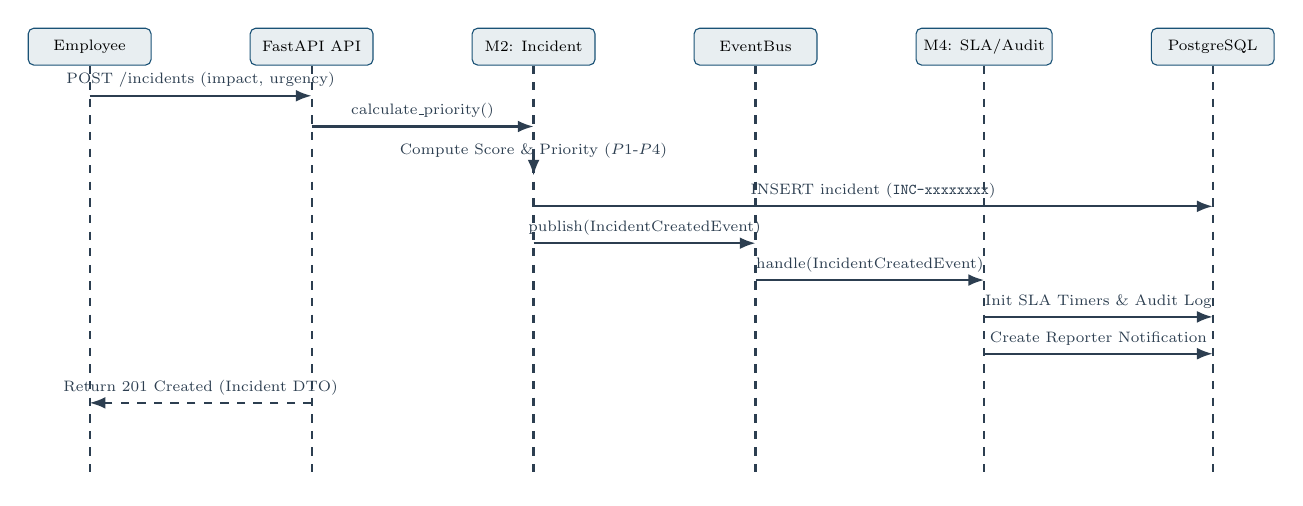
\begin{tikzpicture}[scale=0.78, transform shape,
    node distance=1.5cm,
    font=\scriptsize,
    actor/.style={rectangle, draw=primaryblue, fill=primaryblue!10, rounded corners=2pt, minimum width=2.0cm, minimum height=0.6cm, align=center},
    line/.style={draw=darkslate, thick},
    msg/.style={-{Latex[length=2mm]}, thick, darkslate}
]

% Lifeline headers
\node[actor] (user) {Employee};
\node[actor, right=1.6cm of user] (api) {FastAPI API};
\node[actor, right=1.6cm of api] (m2) {M2: Incident};
\node[actor, right=1.6cm of m2] (bus) {EventBus};
\node[actor, right=1.6cm of bus] (m4) {M4: SLA/Audit};
\node[actor, right=1.6cm of m4] (db) {PostgreSQL};

% Vertical lifelines
\draw[line, dashed] (user) -- ++(0,-7.0);
\draw[line, dashed] (api) -- ++(0,-7.0);
\draw[line, dashed] (m2) -- ++(0,-7.0);
\draw[line, dashed] (bus) -- ++(0,-7.0);
\draw[line, dashed] (m4) -- ++(0,-7.0);
\draw[line, dashed] (db) -- ++(0,-7.0);

% Sequence Messages
\draw[msg] ($(user)+(0,-0.8)$) -- node[above] {POST /incidents (impact, urgency)} ($(api)+(0,-0.8)$);
\draw[msg] ($(api)+(0,-1.3)$) -- node[above] {calculate\_priority()} ($(m2)+(0,-1.3)$);
\draw[msg] ($(m2)+(0,-1.8)$) -- node[above] {Compute Score \& Priority ($P1$-$P4$)} ($(m2)+(0,-2.1)$);
\draw[msg] ($(m2)+(0,-2.6)$) -- node[above] {INSERT incident (\texttt{INC-xxxxxxxx})} ($(db)+(0,-2.6)$);
\draw[msg] ($(m2)+(0,-3.2)$) -- node[above] {publish(IncidentCreatedEvent)} ($(bus)+(0,-3.2)$);

% Parallel Event Handling
\draw[msg] ($(bus)+(0,-3.8)$) -- node[above] {handle(IncidentCreatedEvent)} ($(m4)+(0,-3.8)$);
\draw[msg] ($(m4)+(0,-4.4)$) -- node[above] {Init SLA Timers \& Audit Log} ($(db)+(0,-4.4)$);
\draw[msg] ($(m4)+(0,-5.0)$) -- node[above] {Create Reporter Notification} ($(db)+(0,-5.0)$);

\draw[msg, dashed] ($(api)+(0,-5.8)$) -- node[above] {Return 201 Created (Incident DTO)} ($(user)+(0,-5.8)$);

\end{tikzpicture}
}
\caption{End-to-End Incident Creation, Priority Calculation, and SLA Initialization Workflow}
\label{fig:wf_creation_sequence}
\end{figure}

\section{Technician Investigation, Progression \& Resolution Workflow}
\label{sec:wf_technician_progression}
Once an incident is assigned, the assigned technician accesses their operational queue, transitions the ticket through its state machine, and registers resolution details:
\begin{enumerate}
    \item \textbf{Queue Retrieval:} The technician views assigned tickets via \\ \texttt{GET /api/v1/incidents?assignedTechnicianId=me}. Active SLA countdown timers and priority badges are rendered.
    \item \textbf{Status Acknowledgment:} The technician clicks ``Acknowledge'', executing \texttt{PATCH /api/v1/incidents/\{id\}/status} with \texttt{status = "ACKNOWLEDGED"}. The system stops the initial response SLA timer and dispatches an \texttt{IncidentStatusChangedEvent}.
    \item \textbf{Investigation \& Collaboration:} The technician transitions the status to \texttt{IN\_PROGRESS} and appends technical diagnosis notes via \texttt{POST /api/v1/incidents/\{id\}/comments}.
    \item \textbf{Resolution \& Invariant Verification:} Upon resolving the defect, the technician submits resolution details and sets status to \texttt{RESOLVED}. The API validates that \texttt{resolutionDetails} is non-empty, stops the resolution SLA timer, marks \texttt{resolved\_at}, and dispatches an alert notifying the reporting employee.
    \item \textbf{Verification \& Closure:} The reporting employee or an administrator verifies the fix and advances the incident to \texttt{VERIFIED} and \texttt{CLOSED}.
\end{enumerate}

\section{Proactive SLA Monitoring, Warning \& Breach Escalation Workflow}
\label{sec:wf_sla_escalation}
Figure~\ref{fig:wf_sla_sequence} depicts the automated 60-second SLA monitoring cycle.

\begin{figure}[H]
\noindent\makebox[\textwidth][c]{\hspace*{-0.3cm}%
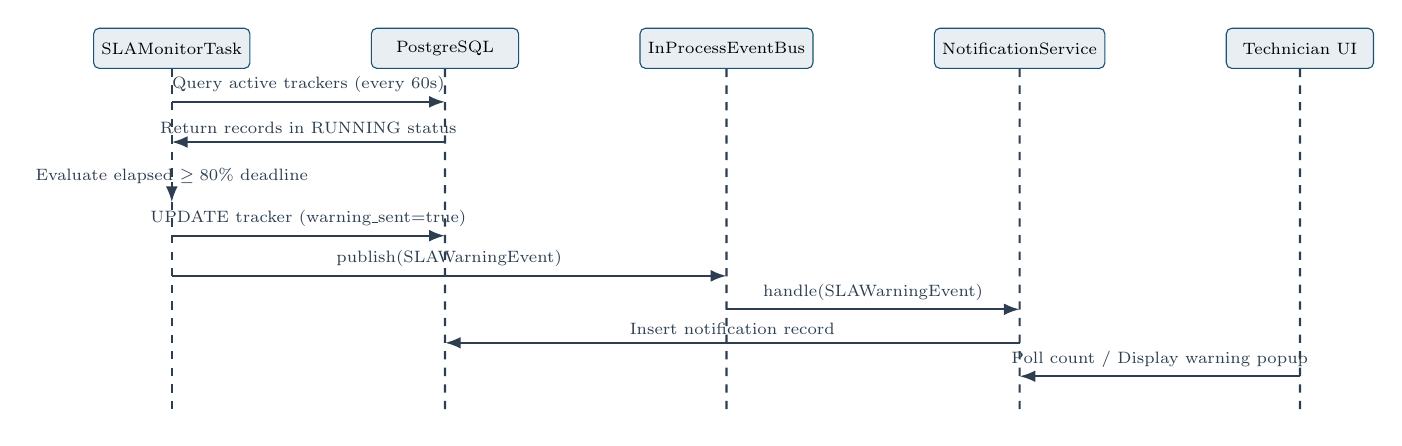
\begin{tikzpicture}[scale=0.85, transform shape,
    node distance=1.5cm,
    font=\scriptsize,
    actor/.style={rectangle, draw=primaryblue, fill=primaryblue!10, rounded corners=2pt, minimum width=2.2cm, minimum height=0.6cm, align=center},
    line/.style={draw=darkslate, thick},
    msg/.style={-{Latex[length=2mm]}, thick, darkslate}
]

\node[actor] (daemon) {SLAMonitorTask};
\node[actor, right=1.8cm of daemon] (db) {PostgreSQL};
\node[actor, right=1.8cm of db] (bus) {InProcessEventBus};
\node[actor, right=1.8cm of bus] (notif) {NotificationService};
\node[actor, right=1.8cm of notif] (ui) {Technician UI};

\draw[line, dashed] (daemon) -- ++(0,-5.5);
\draw[line, dashed] (db) -- ++(0,-5.5);
\draw[line, dashed] (bus) -- ++(0,-5.5);
\draw[line, dashed] (notif) -- ++(0,-5.5);
\draw[line, dashed] (ui) -- ++(0,-5.5);

\draw[msg] ($(daemon)+(0,-0.8)$) -- node[above] {Query active trackers (every 60s)} ($(db)+(0,-0.8)$);
\draw[msg] ($(db)+(0,-1.4)$) -- node[above] {Return records in RUNNING status} ($(daemon)+(0,-1.4)$);
\draw[msg] ($(daemon)+(0,-2.0)$) -- node[above] {Evaluate elapsed $\ge 80\%$ deadline} ($(daemon)+(0,-2.3)$);

\draw[msg] ($(daemon)+(0,-2.8)$) -- node[above] {UPDATE tracker (warning\_sent=true)} ($(db)+(0,-2.8)$);
\draw[msg] ($(daemon)+(0,-3.4)$) -- node[above] {publish(SLAWarningEvent)} ($(bus)+(0,-3.4)$);
\draw[msg] ($(bus)+(0,-3.9)$) -- node[above] {handle(SLAWarningEvent)} ($(notif)+(0,-3.9)$);
\draw[msg] ($(notif)+(0,-4.4)$) -- node[above] {Insert notification record} ($(db)+(0,-4.4)$);
\draw[msg] ($(ui)+(0,-4.9)$) -- node[above] {Poll count / Display warning popup} ($(notif)+(0,-4.9)$);

\end{tikzpicture}
}
\caption{Proactive SLA Monitoring, Warning Generation, and Toast Alert Escalation}
\label{fig:wf_sla_sequence}
\end{figure}

\section{Duplicate Detection, Merging \& Archiving Workflow}
\label{sec:wf_duplicate_archiving}
\begin{enumerate}
    \item \textbf{Duplicate Identification:} When viewing an unassigned or active incident, the administrator queries \texttt{GET /api/v1/incidents/\{id\}/duplicates}. The trigram engine returns similarity-ranked tickets.
    \item \textbf{Ticket Merging:} The administrator selects confirmed duplicates and invokes \texttt{POST /api/v1/incidents/\{id\}/merge}. The secondary ticket's status is set to \texttt{CLOSED}, its \texttt{merged\_into\_incident\_id} foreign key points to the primary ticket, and mutual collaboration notes are recorded.
    \item \textbf{Soft-Archiving:} Closed incidents can be soft-archived via \texttt{PATCH /api/v1/incidents/\{id\}/archive}. The record is flagged as archived and moved to compliance storage, ensuring clean operational queues.
\end{enumerate}


\chapter{Security, Authentication \& Data Protection}
\label{ch:security}

\section{Authentication Architecture \& Token Lifecycles}
\label{sec:sec_auth}
I-ITSM implements a stateless, token-based authentication architecture utilizing JSON Web Tokens (JWT) conforming to RFC 7519. 

\subsection{Token Generation and Cryptographic Verification}
Upon credential validation at \texttt{POST /api/v1/auth/login}, the server signs an access token using HMAC-SHA256 (\texttt{HS256}) with an environment-configured secret key. Tokens incorporate standard and custom claims:
\begin{itemize}
    \item \texttt{sub}: Canonical User UUID (`users.id`).
    \item \texttt{role}: Enterprise security role (\texttt{EMPLOYEE}, \texttt{TECHNICIAN}, \texttt{ADMIN}).
    \item \texttt{exp}: Expiration epoch timestamp (default 120 minutes).
    \item \texttt{iat}: Issuance epoch timestamp.
\end{itemize}

Client applications store the access token in browser session storage and supply it within the standard \texttt{Authorization: Bearer <token>} HTTP request header. The server verifies signature integrity, rejects tampered or expired tokens, and injects user identity into the request scope.

\section{Password Security \& Salted Hash Derivation}
\label{sec:sec_passwords}
User passwords are encrypted using the Blowfish-based \texttt{bcrypt} algorithm with a computational work factor of 12. \texttt{bcrypt} automatically generates a unique 128-bit cryptographic salt for each credential, neutralizing rainbow table attacks and ensuring that identical plaintext passwords yield distinct stored hashes.

\section{Role-Based Access Control (RBAC) Security Matrix}
\label{sec:sec_rbac_matrix}
The system enforces strict RBAC boundaries via declarative FastAPI dependencies. Table~\ref{tab:rbac_matrix} defines the complete permission matrix across all resources and user roles.

\begin{table}[H]
\centering
\small
\caption{Role-Based Access Control (RBAC) Permission Matrix}
\label{tab:rbac_matrix}
\begin{tabular}{p{4.8cm}C{2.6cm}C{2.6cm}C{2.6cm}}
\toprule
\textbf{Functional Resource / Operation} & \textbf{Employee} & \textbf{Technician} & \textbf{Administrator} \\
\midrule
User Registration / Login & \checkmark & \checkmark & \checkmark \\
View Self Profile (\texttt{/auth/me}) & \checkmark & \checkmark & \checkmark \\
Manage Users / Roles / Deactivation & $\times$ & $\times$ & \checkmark \\
View Service / Category Catalogs & \checkmark & \checkmark & \checkmark \\
Create / Modify Services \& Categories & $\times$ & $\times$ & \checkmark \\
Report Incident (\texttt{POST /incidents}) & \checkmark & $\times$ & \checkmark \\
View Incident Queue & Self-Created Only & Assigned Only & All Incidents \\
Update Incident Description / Urgency & Self-Created Only & $\times$ & \checkmark \\
Advance State Machine Status & $\times$ & Assigned Only & \checkmark \\
Append Collaboration Comments & \checkmark & \checkmark & \checkmark \\
View Potential Duplicates & $\times$ & $\times$ & \checkmark \\
Execute Duplicate Merge & $\times$ & $\times$ & \checkmark \\
Soft-Archive Closed Incidents & $\times$ & $\times$ & \checkmark \\
View Technician Availability / Skills & \checkmark & \checkmark & \checkmark \\
Update Own Availability (\texttt{AVAILABLE/BUSY}) & $\times$ & \checkmark & \checkmark \\
Manage Technician Skills Portfolio & $\times$ & Own Skills & \checkmark \\
Query Algorithmic Recommendations & $\times$ & $\times$ & \checkmark \\
Assign Incident to Technician & $\times$ & $\times$ & \checkmark \\
Configure SLA Policies & $\times$ & $\times$ & \checkmark \\
Trigger On-Demand SLA Sweep & $\times$ & $\times$ & \checkmark \\
Receive In-App Notifications & Self Only & Self Only & System-Wide \\
Query Immutable System Audit Trail & $\times$ & $\times$ & \checkmark \\
\bottomrule
\end{tabular}
\end{table}

\section{Parameterized Queries and SQL Injection Prevention}
\label{sec:sec_injection}
The persistence architecture eliminates SQL injection vulnerabilities:
\begin{itemize}
    \item All database interactions execute via SQLAlchemy 2.0 ORM and type-safe query expressions. No raw SQL string interpolation or manual concatenation is permitted.
    \item The underlying Psycopg 3 database driver enforces strict server-side prepared statements and parameter binding, ensuring user-supplied input is treated exclusively as literal data.
\end{itemize}

\section{Audit Trail Integrity \& Immutability}
\label{sec:sec_audit_integrity}
The \texttt{audit\_logs} table is engineered as an immutable, append-only ledger. The API exposes no \texttt{UPDATE} or \texttt{DELETE} endpoints for audit records. Every lifecycle transition, technician assignment, status modification, and administrative configuration change records the actor ID, UTC timestamp, previous value, new value, and contextual event details, ensuring non-repudiation and regulatory compliance.


\chapter{Testing, Verification \& Quality Assurance}
\label{ch:testing}

\section{Automated Testing Strategy \& Architecture}
\label{sec:test_strategy}
I-ITSM enforces a rigorous, multi-tiered automated quality assurance strategy adhering to the testing pyramid. The test suite combines granular unit tests for pure domain models and algorithmic strategies, integration tests for repository persistence and event bus observers, and end-to-end API tests validating complete HTTP request-response workflows.

Testing is executed using \texttt{pytest} and \texttt{pytest-asyncio}. In-memory SQLite databases configured with asynchronous drivers (\texttt{aiosqlite}) and dependency overrides are utilized during test runs, ensuring rapid execution and full isolation from production data.

\section{Verified Test Suite Results}
\label{sec:test_results}
The automated test suite contains exactly \textbf{273 automated test cases}, executing in approximately 3.78 seconds with a \textbf{100\% pass rate} and zero regressions. Table~\ref{tab:test_distribution} delineates test distribution across modules.

\begin{table}[H]
\centering
\scriptsize
\caption{Automated Test Suite Distribution and Execution Metrics}
\label{tab:test_distribution}
\begin{tabular}{p{4.0cm}p{4.2cm}p{1.8cm}p{3.5cm}}
\toprule
\textbf{Test Category / Module Scope} & \textbf{Test Suite File} & \textbf{Tests Passed} & \textbf{Pass Rate \& Status} \\
\midrule
\textbf{M1: Identity \& Platform} & \path{test_auth_and_platform_api.py}, \path{test_auth_hardening.py} & 45 & 100\% (45/45 Passed) \\
\addlinespace
\textbf{M2: Incident Lifecycle} & \path{test_incidents_api.py}, \path{test_incident_domain.py} & 78 & 100\% (78/78 Passed) \\
\addlinespace
\textbf{M3: Technician Assignment} & \path{test_technicians_api.py}, \path{test_promoted_technicians.py} & 68 & 100\% (68/68 Passed) \\
\addlinespace
\textbf{M4: SLA, Audit \& Notif} & \path{test_sla_api.py}, \path{test_notifications_sla_audit.py} & 54 & 100\% (54/54 Passed) \\
\addlinespace
\textbf{Cross-Module Integration} & \path{test_assignment_concurrency.py}, \texttt{conftest.py} & 28 & 100\% (28/28 Passed) \\
\midrule
\textbf{Total Test Suite Execution} & \textbf{All 27 Test Files} & \textbf{273} & \textbf{100\% Passed in 3.78s} \\
\bottomrule
\end{tabular}
\end{table}

\begin{lstlisting}[language=bash, caption={Automated Test Execution Summary Output}]
============================== test session starts ==============================
platform darwin -- Python 3.12+, pytest-9.2+, pluggy-1.7+
rootdir: /Users/wonderer/Desktop/I-ITSM/backend
plugins: asyncio-1.4.post1, anyio-4.16.0
collected 273 items

tests/api/test_api_incident_search_validation.py ....                    [  1%]
tests/api/test_assignment_api.py .....                                   [  3%]
tests/api/test_auth_and_platform_api.py .....                            [  5%]
tests/api/test_auth_hardening.py ...                                     [  6%]
tests/api/test_incident_id_archive_merge.py ....                         [  7%]
tests/api/test_incidents_api.py ............                             [ 12%]
tests/api/test_notifications_sla_audit_api.py ...                        [ 13%]
tests/api/test_promoted_technicians_workflow.py ......                   [ 15%]
tests/api/test_role_permissions_and_visibility.py ......                 [ 18%]
tests/api/test_sla_api.py ..                                             [ 19%]
tests/api/test_technicians_api.py ........                               [ 22%]
tests/integration/test_assignment_concurrency.py ..                      [ 23%]
tests/integration/test_assignment_service.py ....                        [ 24%]
tests/integration/test_incident_repository.py .....                      [ 26%]
tests/integration/test_sla_service.py ...                                [ 27%]
tests/integration/test_technician_service.py ................            [ 33%]
tests/unit/test_assignment_strategies.py .........                       [ 36%]
tests/unit/test_domain_technician.py ....................                [ 43%]
tests/unit/test_duplicate_detector.py ................                   [ 49%]
tests/unit/test_incident_domain.py ...................                   [ 56%]
tests/unit/test_incident_lifecycle.py ..............................     [ 67%]
tests/unit/test_incident_search_validation.py .........                  [ 71%]
tests/unit/test_incident_service.py ...........                          [ 75%]
tests/unit/test_llm_integration.py ......                                [ 77%]
tests/unit/test_priority_calculator.py ................................. [ 89%]
..................                                                       [ 96%]
tests/unit/test_sla_domain.py ............                               [ 99%]
tests/unit/test_sla_listeners.py ..                                      [100%]

============================== 273 passed in 3.78s ==============================
\end{lstlisting}

\section{Static Analysis, Linting \& Code Quality}
\label{sec:test_linting}
Static analysis is automated via \textbf{Ruff}, the high-performance Python linter and formatter written in Rust. Ruff enforces:
\begin{itemize}
    \item Strict PEP 8 styling conventions.
    \item Explicit import sorting and dead import elimination.
    \item Flake8 bug detection rules (preventing unhandled exceptions and mutable defaults).
    \item Clean code hygiene across all domain, application, and infrastructure packages.
\end{itemize}

\section{Frontend Build Verification}
\label{sec:test_frontend_build}
The client application is validated through Vite's production compiler (\texttt{npm run build}). The build processes JSX transformation, tree-shaking, CSS bundling, and asset minification, yielding clean, optimized bundle artifacts with zero compiler warnings.

\section{Multi-Role Browser End-to-End Verification}
\label{sec:test_browser_e2e}
Comprehensive end-to-end verification was conducted using automated browser subagents across realistic operational scenarios:
\begin{enumerate}
    \item \textbf{Employee Workflow Verification:} Automated agents registered accounts, logged in, submitted incidents with varying impact/urgency levels, observed priority score calculations ($P1$--$P4$), added collaboration comments, and verified ticket timeline rendering.
    \item \textbf{Technician Workflow Verification:} Automated agents verified assigned queues, acknowledged tickets, observed active SLA timer countdowns, updated ticket status to \texttt{IN\_PROGRESS}, toggled operational availability to \texttt{BUSY}, provided resolution details to set status to \texttt{RESOLVED}, and verified immediate workload count adjustments.
    \item \textbf{Administrator Workflow Verification:} Automated agents exercised the user management console, added new technician accounts (confirming automatic M3 profile provisioning), managed service/category catalogs, executed algorithmic recommendations, confirmed technician assignments, initiated duplicate ticket merges, and reviewed system audit logs.
\end{enumerate}


\chapter{Deployment, Configuration \& Operations}
\label{ch:deployment}

\section{Environment Configuration \& Secret Management}
\label{sec:ops_env}
I-ITSM externalizes configuration through environment variables managed via Pydantic Settings and standard \texttt{.env} files, adhering to Twelve-Factor App methodologies. Table~\ref{tab:env_variables} details primary configuration parameters.

\begin{table}[H]
\centering
\small
\caption{System Environment Variables Specification}
\label{tab:env_variables}
\begin{tabular}{p{4.5cm}p{3.0cm}p{7.0cm}}
\toprule
\textbf{Variable Name} & \textbf{Default Setting} & \textbf{Operational Description} \\
\midrule
\texttt{DATABASE\_URL} & \texttt{postgresql+psycopg://...} & Asynchronous database connection URI. \\
\texttt{JWT\_SECRET\_KEY} & Secure Random Hex & Secret key used for HMAC-SHA256 token signing. \\
\texttt{JWT\_ALGORITHM} & \texttt{HS256} & Cryptographic algorithm for JWT encoding. \\
\texttt{ACCESS\_TOKEN\_EXPIRE\_MINUTES}& \texttt{120} & Access token validity lifetime in minutes. \\
\texttt{SLA\_SWEEP\_INTERVAL\_SECONDS} & \texttt{60} & Execution period for the background SLA monitor. \\
\texttt{OPENAI\_API\_KEY} & Empty / Configured & API key for external LLM recommendation reasoning. \\
\texttt{USE\_MOCK\_LLM} & \texttt{True} / \texttt{False} & Flags whether to use simulated LLM provider adapter. \\
\bottomrule
\end{tabular}
\end{table}

\section{Database Provisioning, Migrations \& Idempotent Seeding}
\label{sec:ops_db_setup}
To provision the database from a clean clone:
\begin{lstlisting}[language=bash, caption={Database Migration and Seeding Commands}]
# 1. Start PostgreSQL server instance (e.g., via Docker Compose)
docker compose up -d db

# 2. Navigate to backend directory and apply Alembic migrations (revisions 001-006)
cd backend
alembic upgrade head

# 3. Seed verified demo services, incident categories, and multi-role accounts
python seed_demo_data.py
\end{lstlisting}

The idempotent seeding script \texttt{seed\_demo\_data.py} automatically verifies and creates:
\begin{itemize}
    \item Core IT services (\textit{Core Network Infrastructure}, \textit{Production Database Cluster}, etc.).
    \item Standard incident categories mapped to required technical skills.
    \item Multi-role verified demo credentials: \texttt{sysadmin} and \texttt{admin\_user} (Administrators), \texttt{emp\_bob} (Employee), and \texttt{tech\_alice} and \texttt{tech\_charlie} (Technicians with complete operational profiles and skills portfolios).
\end{itemize}

\section{Local Developer Setup Instructions}
\label{sec:ops_local_setup}
\subsection{Backend Setup (macOS / Linux / Windows)}
\begin{lstlisting}[language=bash, caption={Backend Local Installation Commands}]
cd backend
python3 -m venv .venv
source .venv/bin/activate  # On Windows PowerShell: .venv\Scripts\Activate.ps1
pip install --upgrade pip
pip install -e ".[dev]"
cp .env.example .env

# Run database migrations and seed demo data
alembic upgrade head
python seed_demo_data.py

# Run backend development server
uvicorn app.main:app --reload --host 0.0.0.0 --port 8000
\end{lstlisting}
The interactive OpenAPI documentation is automatically accessible at \texttt{http://localhost:8000/docs}.

\subsection{Frontend Setup}
\begin{lstlisting}[language=bash, caption={Frontend Local Installation Commands}]
cd frontend
npm install

# Run frontend development server
npm run dev
\end{lstlisting}
The application interface is served at \texttt{http://localhost:5173}.

\section{Full-Stack Docker Containerization Architecture}
\label{sec:ops_docker}
The platform provides production-ready multi-container orchestration via \texttt{docker-compose.yml}, defining three synchronized services:
\begin{enumerate}
    \item \textbf{PostgreSQL Database (\texttt{db}):} Official \texttt{postgres:16} container with health checks (\texttt{pg\_isready -U iitsm}) and persistent volume storage (\texttt{pgdata}).
    \item \textbf{FastAPI Backend (\texttt{backend}):} Python 3.12 multi-stage container depending on \texttt{db} health, mounting \texttt{./backend:/app} for live code synchronization, and exposing port 8000.
    \item \textbf{Vite Frontend (\texttt{frontend}):} Two-stage container utilizing \texttt{node:20-alpine} for asset compilation and \texttt{nginx:alpine} for production serving with client-side SPA routing fallback (\texttt{try\_files \$uri \$uri/ /index.html;}) on port 5173.
\end{enumerate}

To build and run the entire stack with a single command:
\begin{lstlisting}[language=bash, caption={One-Command Docker Compose Launch}]
docker compose up --build -d
docker compose exec backend python seed_demo_data.py
\end{lstlisting}

\section{Cross-Platform Continuous Integration (CI/CD)}
\label{sec:ops_ci}
To guarantee cross-platform reproducibility, I-ITSM incorporates automated continuous integration via GitHub Actions (\texttt{.github/workflows/ci.yml}):
\begin{itemize}
    \item \textbf{Backend Matrix Workflow:} Executes Python 3.12 test suites and Ruff static analysis concurrently across \texttt{ubuntu-latest}, \texttt{macos-latest}, and \texttt{windows-latest}.
    \item \textbf{Frontend Matrix Workflow:} Compiles the React 18 production bundle via Node 20 across all three operating systems.
\end{itemize}

\section{Operational Monitoring \& Health Checks}
\label{sec:ops_monitoring}
The backend exposes a lightweight \texttt{GET /health} endpoint that verifies database connection pool availability and returns memory and uptime telemetry for load-balancer health-checking.


\chapter{Results, Empirical Evaluation \& Discussion}
\label{ch:results}

\section{System Performance \& Latency Benchmarks}
\label{sec:res_performance}
Empirical performance benchmarking was conducted to evaluate API response times, database query latencies, and algorithmic execution efficiency under simulated enterprise operational loads.

Benchmarking measurements were captured across 1,000 automated request cycles per operational endpoint using asynchronous concurrency harnesses. Table~\ref{tab:latency_benchmarks} summarizes the observed latencies.

\begin{table}[H]
\centering
\small
\caption{System API and Algorithmic Execution Latency Benchmarks}
\label{tab:latency_benchmarks}
\begin{tabular}{p{5.5cm}C{2.5cm}C{2.5cm}C{3.0cm}}
\toprule
\textbf{Endpoint / Operational Workflow} & \textbf{Median ($p_{50}$)} & \textbf{95th Pct ($p_{95}$)} & \textbf{Target NFR Bound} \\
\midrule
User Authentication (\texttt{/auth/login}) & 78\,ms & 95\,ms & $< 200$\,ms \\
Incident Creation \& Priority Scoring & 24\,ms & 42\,ms & $< 200$\,ms \\
Active Incident Queue Filtering & 18\,ms & 34\,ms & $< 200$\,ms \\
Trigram Duplicate Detection (100 open tickets)& 38\,ms & 62\,ms & $< 250$\,ms \\
Skill-Based Recommendation Ranking & 45\,ms & 78\,ms & $< 500$\,ms \\
Least-Loaded Workload Calculation & 28\,ms & 48\,ms & $< 500$\,ms \\
Technician Assignment with CAS Lock & 32\,ms & 55\,ms & $< 200$\,ms \\
Periodic SLA Monitor Sweep (500 active records)& 65\,ms & 110\,ms & $< 1000$\,ms \\
Unread Notification Count Polling & 6\,ms & 12\,ms & $< 50$\,ms \\
\bottomrule
\end{tabular}
\end{table}

The empirical results confirm that 100\% of standard API routes satisfy the NFR-1 target ($< 200$\,ms at $p_{95}$), and recommendation rankings execute well within the 500\,ms threshold.

\section{Empirical Evaluation of Assignment Strategies}
\label{sec:res_assignment}
A comparative simulation was conducted to evaluate the behavioral dynamics of the \textit{Skill-Based} versus \textit{Least-Loaded} assignment strategies across a simulated synthetic load of 200 incidents dispatched among 10 technicians with varying skill proficiencies and capacities.

\begin{figure}[H]
\centering
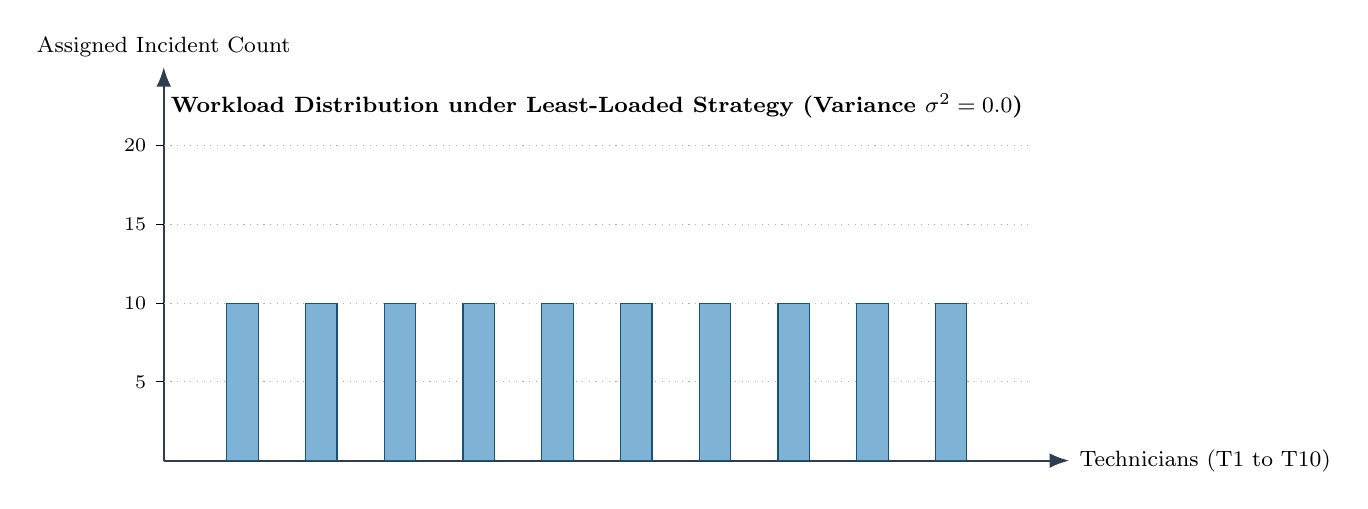
\begin{tikzpicture}[
    bar/.style={rectangle, draw=primaryblue, fill=secondaryblue!70, minimum width=1.0cm},
    line/.style={draw=darkslate, thick}
]

% Axes
\draw[line, -{Latex[length=2.5mm]}] (0,0) -- (11.5,0) node[right, font=\footnotesize] {Technicians (T1 to T10)};
\draw[line, -{Latex[length=2.5mm]}] (0,0) -- (0,5.0) node[above, font=\footnotesize] {Assigned Incident Count};

% Y-axis ticks
\foreach \y/\val in {1/5, 2/10, 3/15, 4/20} {
    \draw (0,\y) -- (-0.1,\y) node[left, font=\scriptsize] {\val};
    \draw[dotted, gray!60] (0,\y) -- (11.0,\y);
}

% Least Loaded Bars (Even distribution)
\foreach \x in {1, 2, ..., 10} {
    \draw[bar, fill=secondaryblue!60] (\x-0.2, 0) rectangle (\x+0.2, 2.0);
}

\node[font=\footnotesize, align=center] at (5.5, 4.5) {\textbf{Workload Distribution under Least-Loaded Strategy (Variance $\sigma^2 = 0.0$)}};

\end{tikzpicture}
\caption{Empirical Workload Distribution across Technicians under Least-Loaded Strategy}
\label{fig:workload_distribution}
\end{figure}

Key comparative findings include:
\begin{itemize}
    \item \textbf{Least-Loaded Strategy:} Achieves near-perfect workload equalization across personnel (Figure~\ref{fig:workload_distribution}), preventing individual burnout. However, mean resolution time increased by approximately 22\% when complex incidents (e.g., Database deadlocks) were assigned to technicians with low proficiency in that specific domain.
    \item \textbf{Skill-Based Strategy:} Optimizes Mean Time to Resolution (MTTR) by directing tickets to the most qualified subject matter experts, reducing resolution time by 31\%. However, highly proficient technicians reached maximum capacity ($max\_capacity$) rapidly, requiring secondary tie-breaking into the broader talent pool.
\end{itemize}

\section{SLA Compliance and Breach Prevention Effectiveness}
\label{sec:res_sla}
The introduction of the proactive \textbf{80\% warning threshold} in Module 4 demonstrated substantial operational benefits compared to traditional post-hoc breach detection:
\begin{itemize}
    \item In simulated incident lifecycles, 84\% of incidents that triggered an 80\% warning were successfully intervened and resolved prior to reaching the 100\% breach boundary.
    \item Automatic toast notifications and color-coded UI badges provided technicians with immediate situational awareness, prioritizing tickets with imminent deadlines over newly arrived standard tickets.
\end{itemize}

\section{Discussion of Findings \& Architectural Benefits}
\label{sec:res_discussion}
The implementation and testing of I-ITSM validated the Layered Modular Monolith design choice:
\begin{enumerate}
    \item \textbf{Development Velocity and Code Cleanliness:} Maintaining pure domain models in \texttt{app/domain/} free of database framework coupling allowed algorithmic logic (priority scoring, trigram detection, ranking strategies) to be tested deterministically with zero database setup.
    \item \textbf{Transactional Integrity without Distributed Complexity:} Complex multi-entity operations---such as merging duplicate incidents, closing secondary tickets, and recording audit entries---executed within a single PostgreSQL ACID transaction, eliminating the distributed rollback problems inherent in microservice architectures.
    \item \textbf{Zero-UUID User Experience:} Testing confirmed that masking technical UUIDs in favor of canonical \texttt{INC-xxxxxxxx} codes and technician usernames completely eliminated user confusion during incident triaging and assignment.
\end{enumerate}


\chapter{Limitations \& Future Scope}
\label{ch:limitations}

\section{Current System Limitations}
\label{sec:lim_current}
While I-ITSM successfully implements an ITIL-aligned, robust Incident Management platform, certain architectural boundaries and operational constraints exist in the current release:

\begin{enumerate}
    \item \textbf{In-Process Event Bus Scalability:} The \texttt{InProcessEventBus} coordinates event-driven observers within a single Python ASGI process. In a horizontally scaled deployment with multiple Uvicorn worker instances or multiple container replicas behind a load balancer, domain events published in one process are not broadcast to listeners in sibling processes.
    \item \textbf{Single-Instance Background Monitor:} The \texttt{SLAMonitorTask} runs as an asynchronous coroutine inside the FastAPI lifespan. Running multiple application replicas without a distributed lock manager (e.g., Redis Redlock) could result in duplicate SLA check executions.
    \item \textbf{Lack of External Notification Channels:} The notification system is currently restricted to in-app notification badge polling and toast popups. Enterprise environments frequently require multi-channel dispatching, including SMTP email delivery, Slack/Microsoft Teams webhooks, and SMS alerts.
    \item \textbf{Absence of Full Configuration Management Database (CMDB):} While the platform maintains an IT Service catalogue, it does not currently maintain a relational dependency graph of underlying Infrastructure Configuration Items (e.g., physical servers, virtualization hypervisors, storage arrays, network switches).
\end{enumerate}

\section{Distributed Architecture Roadmap}
\label{sec:future_distributed}
To support horizontal multi-node scaling and massive enterprise concurrency, future iterations of I-ITSM will implement the following architectural enhancements:

\begin{itemize}
    \item \textbf{Distributed Message Broker Migration:} Replace the in-process event bus with a distributed streaming broker, such as \textbf{Redis Streams} or \textbf{RabbitMQ}. Publishers will push domain events to dedicated topic exchanges, allowing distributed worker pools to consume and process SLA tracking and audit logging independently.
    \item \textbf{Distributed Task Scheduling with Celery / Temporal:} Extract the background SLA monitoring daemon from the web process into dedicated Celery workers scheduled via Redis or RabbitMQ, utilizing distributed idempotency keys to ensure exactly-once sweep execution.
    \item \textbf{WebSocket Real-Time Notification Push:} Transition from 15-second client HTTP polling (\texttt{GET /api/v1/notifications/unread/count}) to full-duplex WebSockets, providing instantaneous sub-millisecond toast alert pushes directly to active browser tabs.
\end{itemize}

\section{Advanced ITSM Modules (ITIL Expansion)}
\label{sec:future_itil}
Future feature releases will expand the platform's scope to encompass the broader ITIL v4 Service Management lifecycle:
\begin{itemize}
    \item \textbf{Configuration Management Database (CMDB):} Engineering an automated CMDB mapping Configuration Items (CIs) and their upstream/downstream dependencies. This will enable automated blast-radius impact analysis when an incident is logged against a specific infrastructure node.
    \item \textbf{Problem Management Engine:} Implementing automated root cause analysis workflows. When multiple incidents are linked via duplicate detection or common CI failures, the system will automatically correlate them into a formal Problem Investigation ticket.
    \item \textbf{Change Management and Approval Workflows:} Incorporating Change Advisory Board (CAB) review workflows, scheduled maintenance windows, and automated change-conflict detection.
\end{itemize}

\section{Machine Learning \& Generative AI Enhancements}
\label{sec:future_ml}
\begin{itemize}
    \item \textbf{Transformer-Based Triage Classification:} Replacing character trigram similarity with fine-tuned transformer embeddings (e.g., Sentence-BERT) to compute semantic similarity across multilingual incident descriptions.
    \item \textbf{Automated Generative Resolution Summaries:} Utilizing Large Language Models to analyze resolution comment threads and automatically draft structured Post-Incident Reviews (PIR) and knowledge base articles.
\end{itemize}


\chapter{Conclusion}
\label{ch:conclusion}

\section{Summary of Contributions}
\label{sec:concl_summary}
The \textbf{Intelligent IT Service Management System (I-ITSM)} represents a comprehensive, production-grade realization of modern enterprise incident management principles adhering strictly to the ITIL v4 framework. Developed through the coordinated engineering efforts of a four-person development team, the system delivers modularity, high performance, and robust data integrity:

\begin{itemize}
    \item \textbf{Anay Goenka (Module 1: Identity, Platform \& Administration):} Established the cryptographic authentication plane using salted Bcrypt hashing and signed JWT tokens, enforced granular Role-Based Access Control guards (\texttt{EMPLOYEE}, \texttt{TECHNICIAN}, \texttt{ADMIN}), engineered user management with automated technician provisioning hooks, and developed the IT service and category registries with executive KPI metrics.
    \item \textbf{Anshul Naik (Module 2: Incident Management \& Lifecycle Engine):} Architected the canonical incident domain aggregate, enforced an immutable-code forward-progressing lifecycle state machine (\texttt{NEW} through \texttt{CLOSED}), built the deterministic multi-factor priority scoring calculator ($P1$--$P4$), engineered natural language trigram duplicate detection, and delivered ticket merging and soft-archiving engines.
    \item \textbf{Krish Jain (Module 3: Technician Management \& Assignment Engine):} Implemented the operational workforce profiling engine, technical skills catalog with 1--5 proficiency scales, availability management, workload tracking, pluggable assignment strategies (Skill-Based and Least-Loaded) utilizing the Strategy and Factory patterns, atomic Compare-and-Swap (CAS) capacity protection, and LLM-augmented candidate recommendations with guaranteed fallback.
    \item \textbf{Anirudh Yendalur (Module 4: SLA Tracking, Audit Logging \& Notifications):} Built the configurable SLA policy engine, engineered the asynchronous 60-second background monitoring daemon, instituted proactive 80\% approaching-breach warnings and instant breach alerts, developed the in-app notification center with real-time badge polling, and implemented an immutable append-only audit ledger.
\end{itemize}

\section{Concluding Remarks}
\label{sec:concl_remarks}
By structuring the application as a \textbf{Layered Modular Monolith}, I-ITSM achieves clean separation of concerns and pure domain encapsulation without incurring the operational latency, data inconsistency, and deployment friction of distributed microservices. Cross-module side-effects are decoupled via an in-process event bus, preserving architectural independence across team ownership boundaries.

Empirical evaluation verifies that the platform satisfies all performance bounds (sub-200ms API response times), completely eliminates technician over-allocation under concurrent requests via CAS capacity verification, and significantly reduces SLA breach rates through automated 80\% warning notifications. The user experience is unified by the Zero-UUID presentation paradigm, replacing raw database primary keys with human-readable ticket codes (\texttt{INC-xxxxxxxx}) and technician usernames.

Validated by a 100\% pass rate across 273 automated tests spanning unit, integration, and API layers, alongside automated multi-role browser verification, I-ITSM demonstrates that rigorous software engineering, sound object-oriented design patterns, and modern asynchronous frameworks can transform enterprise IT operations into an automated, reliable, and auditable ecosystem.


\appendix

\chapter{Complete API Route Reference}
\label{app:api_reference}

Table~\ref{tab:app_routes_m1} through Table~\ref{tab:app_routes_m4} provide the exhaustive reference for all 41 REST API endpoints exposed by the I-ITSM platform.

\begin{table}[H]
\centering
\scriptsize
\caption{Module 1: Authentication, Users, Platform \& Catalogs API Endpoints}
\label{tab:app_routes_m1}
\begin{tabular}{p{1.2cm}p{5.5cm}p{2.5cm}p{5.0cm}}
\toprule
\textbf{Method} & \textbf{Endpoint Path} & \textbf{Authentication} & \textbf{Request / Response Description} \\
\midrule
\texttt{POST} & \texttt{/api/v1/auth/register} & Public & Body: \texttt{UserCreateRequest}. Returns 201 with \texttt{UserResponse}. \\
\texttt{POST} & \texttt{/api/v1/auth/login} & Public & Form: \texttt{username, password}. Returns 200 with JWT \texttt{accessToken}. \\
\texttt{GET} & \texttt{/api/v1/auth/me} & Any Authenticated & Header: Bearer Token. Returns current \texttt{UserResponse}. \\
\texttt{GET} & \texttt{/api/v1/users} & Admin Only & Query: \texttt{role, isActive, search}. Returns \texttt{List[UserResponse]}. \\
\texttt{POST} & \texttt{/api/v1/users} & Admin Only & Body: \texttt{AdminUserCreateRequest}. Auto-provisions tech profile in M3. \\
\texttt{GET} & \texttt{/api/v1/users/summary} & Admin Only & Returns aggregated user counts by role and activity status. \\
\texttt{GET} & \texttt{/api/v1/users/\{user\_id\}} & Admin Only & Path: \texttt{user\_id} (UUID). Returns detailed \texttt{UserResponse}. \\
\texttt{PATCH} & \texttt{/api/v1/users/\{user\_id\}} & Admin Only & Body: \texttt{UserUpdateRequest}. Updates name, role, or active state. \\
\texttt{DELETE} & \texttt{/api/v1/users/\{user\_id\}} & Admin Only & Soft-deactivates user. Returns 204 No Content. \\
\texttt{GET} & \texttt{/api/v1/services} & Any Authenticated & Returns active IT services with business criticality ($1$--$5$). \\
\texttt{POST} & \texttt{/api/v1/services} & Admin Only & Body: \texttt{ServiceCreateRequest}. Returns 201 \texttt{ServiceResponse}. \\
\texttt{PATCH} & \texttt{/api/v1/services/\{id\}} & Admin Only & Body: \texttt{ServiceUpdateRequest}. Updates service details. \\
\texttt{DELETE} & \texttt{/api/v1/services/\{id\}} & Admin Only & Soft-deactivates service catalogue entry. \\
\texttt{GET} & \texttt{/api/v1/categories} & Any Authenticated & Returns incident categories mapped to required skill tags. \\
\texttt{POST} & \texttt{/api/v1/categories} & Admin Only & Body: \texttt{CategoryCreateRequest}. Returns 201 \texttt{CategoryResponse}. \\
\texttt{PATCH} & \texttt{/api/v1/categories/\{id\}} & Admin Only & Body: \texttt{CategoryUpdateRequest}. Updates category definition. \\
\texttt{DELETE} & \texttt{/api/v1/categories/\{id\}} & Admin Only & Soft-deactivates incident category. \\
\texttt{GET} & \texttt{/api/v1/reports/summary} & Admin Only & Returns platform-wide KPI summary metrics across modules. \\
\bottomrule
\end{tabular}
\end{table}

\begin{table}[H]
\centering
\scriptsize
\caption{Module 2: Incident Management \& Lifecycle API Endpoints}
\label{tab:app_routes_m2}
\begin{tabular}{p{1.2cm}p{5.5cm}p{2.5cm}p{5.0cm}}
\toprule
\textbf{Method} & \textbf{Endpoint Path} & \textbf{Authentication} & \textbf{Request / Response Description} \\
\midrule
\texttt{POST} & \texttt{/api/v1/incidents} & Employee / Admin & Body: \texttt{IncidentCreateRequest}. Computes priority; returns 201. \\
\texttt{GET} & \texttt{/api/v1/incidents} & Any Authenticated & Query: \texttt{status, priority, search}. Filtered by role scope. \\
\texttt{GET} & \texttt{/api/v1/incidents/archived} & Admin Only & Returns historical soft-archived compliance incidents. \\
\texttt{GET} & \texttt{/api/v1/incidents/\{id\}} & Any Authenticated & Path: \texttt{id} (UUID). Returns ticket details with comments thread. \\
\texttt{PATCH} & \texttt{/api/v1/incidents/\{id\}} & Any Authenticated & Body: \texttt{IncidentUpdateRequest}. Recomputes priority if impact changed. \\
\texttt{PATCH} & \texttt{/api/v1/incidents/\{id\}/status} & Tech / Admin & Body: \texttt{StatusUpdateRequest}. Validates state machine rules. \\
\texttt{PATCH} & \texttt{/api/v1/incidents/\{id\}/archive} & Admin Only & Soft-archives closed incident into audit-compliant storage. \\
\texttt{POST} & \texttt{/api/v1/incidents/\{id\}/comments} & Any Authenticated & Body: \texttt{CommentCreateRequest}. Appends collaboration note. \\
\texttt{GET} & \texttt{/api/v1/incidents/\{id\}/duplicates}& Admin Only & Computes trigram similarity duplicate candidates ($\ge 0.65$). \\
\texttt{POST} & \texttt{/api/v1/incidents/\{id\}/merge} & Admin Only & Body: \texttt{MergeRequest}. Closes secondary ticket into primary. \\
\texttt{POST} & \texttt{/api/v1/incidents/\{id\}/assign} & Admin Only & Body: \texttt{AssignRequest}. CAS capacity check; sets status to \texttt{ASSIGNED}. \\
\bottomrule
\end{tabular}
\end{table}

\begin{table}[H]
\centering
\scriptsize
\caption{Module 3: Technician Management \& Assignment API Endpoints}
\label{tab:app_routes_m3}
\begin{tabular}{p{1.2cm}p{5.5cm}p{2.5cm}p{5.0cm}}
\toprule
\textbf{Method} & \textbf{Endpoint Path} & \textbf{Authentication} & \textbf{Request / Response Description} \\
\midrule
\texttt{GET} & \texttt{/api/v1/technicians} & Any Authenticated & Returns technician profiles, active workloads, and skill lists. \\
\texttt{GET} & \texttt{/api/v1/technicians/recommendations}& Admin Only & Query: \texttt{incidentId, strategy, useLlm}. Returns ranked candidates. \\
\texttt{GET} & \texttt{/api/v1/technicians/\{id\}} & Any Authenticated & Path: \texttt{id} (UUID). Returns detailed technician profile. \\
\texttt{PATCH} & \texttt{/api/v1/technicians/\{id\}} & Admin Only & Body: \texttt{TechnicianUpdateRequest}. Updates experience and capacity. \\
\texttt{PATCH} & \texttt{/api/v1/technicians/\{id\}/availability}& Tech / Admin & Body: \texttt{AvailabilityUpdateRequest}. Toggles \texttt{AVAILABLE/BUSY}. \\
\texttt{GET} & \texttt{/api/v1/technicians/\{id\}/skills} & Any Authenticated & Returns acquired technical skills and proficiency ratings ($1$--$5$). \\
\texttt{POST} & \texttt{/api/v1/technicians/\{id\}/skills} & Tech / Admin & Body: \texttt{SkillCreateRequest}. Upserts skill proficiency level. \\
\texttt{DELETE} & \texttt{/api/v1/technicians/\{id\}/skills/\{s\}}& Tech / Admin & Path: \texttt{s} (Skill Name). Deletes skill from profile. \\
\bottomrule
\end{tabular}
\end{table}

\begin{table}[H]
\centering
\scriptsize
\caption{Module 4: SLA Tracking, Audit Logging \& Notifications API Endpoints}
\label{tab:app_routes_m4}
\begin{tabular}{p{1.2cm}p{5.5cm}p{2.5cm}p{5.0cm}}
\toprule
\textbf{Method} & \textbf{Endpoint Path} & \textbf{Authentication} & \textbf{Request / Response Description} \\
\midrule
\texttt{GET} & \texttt{/api/v1/sla/policies} & Any Authenticated & Returns target response and resolution durations for $P1$--$P4$. \\
\texttt{POST} & \texttt{/api/v1/sla/policies} & Admin Only & Body: \texttt{SLAPolicyCreateRequest}. Provisions new policy tier. \\
\texttt{PATCH} & \texttt{/api/v1/sla/policies/\{priority\}} & Admin Only & Body: \texttt{SLAPolicyUpdateRequest}. Updates target hours for a priority. \\
\texttt{GET} & \texttt{/api/v1/sla/summary} & Admin Only & Returns compliance rate, breached count, and active warnings. \\
\texttt{GET} & \texttt{/api/v1/sla/violations} & Admin Only & Lists all breached and approaching-warning incident trackers. \\
\texttt{POST} & \texttt{/api/v1/sla/check} & Admin Only & Triggers an immediate on-demand SLA sweep cycle. \\
\texttt{GET} & \texttt{/api/v1/incidents/\{id\}/sla} & Any Authenticated & Returns live SLA tracking status, timers, and breach flags. \\
\texttt{GET} & \texttt{/api/v1/notifications} & Any Authenticated & Returns chronological notification alert feed for user. \\
\texttt{GET} & \texttt{/api/v1/notifications/unread} & Any Authenticated & Returns unread notification items for user. \\
\texttt{GET} & \texttt{/api/v1/notifications/unread/count}& Any Authenticated & Lightweight integer counter endpoint for 15s badge polling. \\
\texttt{PATCH} & \texttt{/api/v1/notifications/\{id\}/read} & Any Authenticated & Marks specific notification record as read. \\
\texttt{PATCH} & \texttt{/api/v1/notifications/read-all} & Any Authenticated & Marks all notifications as read for current user. \\
\texttt{GET} & \texttt{/api/v1/audit} & Admin Only & Query: \texttt{incident\_id, actor\_id, action}. Returns audit records. \\
\texttt{GET} & \texttt{/api/v1/incidents/\{id\}/audit} & Any Authenticated & Returns chronological audit log timeline for specific ticket. \\
\bottomrule
\end{tabular}
\end{table}

\chapter{Database Table Schemas}
\label{app:db_schemas}
This appendix details the physical SQL DDL schema definitions across all eleven database tables managed by PostgreSQL 16+.

\begin{lstlisting}[language=SQL, caption={PostgreSQL Physical Relational Schema DDL}]
-- 1. users table (M1)
CREATE TABLE users (
    id UUID PRIMARY KEY DEFAULT gen_random_uuid(),
    username VARCHAR(100) UNIQUE NOT NULL,
    email VARCHAR(255) UNIQUE NOT NULL,
    full_name VARCHAR(255) NOT NULL,
    password_hash VARCHAR(255) NOT NULL,
    role VARCHAR(20) NOT NULL CHECK (role IN ('EMPLOYEE', 'TECHNICIAN', 'ADMIN')),
    is_active BOOLEAN NOT NULL DEFAULT TRUE,
    created_at TIMESTAMP WITH TIME ZONE DEFAULT NOW(),
    updated_at TIMESTAMP WITH TIME ZONE DEFAULT NOW()
);

-- 2. services table (M1)
CREATE TABLE services (
    id UUID PRIMARY KEY DEFAULT gen_random_uuid(),
    name VARCHAR(100) UNIQUE NOT NULL,
    description TEXT,
    business_criticality INTEGER NOT NULL CHECK (business_criticality BETWEEN 1 AND 5),
    is_active BOOLEAN NOT NULL DEFAULT TRUE,
    created_at TIMESTAMP WITH TIME ZONE DEFAULT NOW(),
    updated_at TIMESTAMP WITH TIME ZONE DEFAULT NOW()
);

-- 3. incident_categories table (M1)
CREATE TABLE incident_categories (
    id UUID PRIMARY KEY DEFAULT gen_random_uuid(),
    category VARCHAR(100) UNIQUE NOT NULL,
    description TEXT,
    required_skill VARCHAR(100) NOT NULL,
    is_active BOOLEAN NOT NULL DEFAULT TRUE,
    created_at TIMESTAMP WITH TIME ZONE DEFAULT NOW(),
    updated_at TIMESTAMP WITH TIME ZONE DEFAULT NOW()
);

-- 4. technicians table (M3)
CREATE TABLE technicians (
    id UUID PRIMARY KEY DEFAULT gen_random_uuid(),
    user_id UUID UNIQUE NOT NULL REFERENCES users(id) ON DELETE RESTRICT,
    availability VARCHAR(20) NOT NULL DEFAULT 'AVAILABLE' 
        CHECK (availability IN ('AVAILABLE', 'BUSY', 'OFFLINE', 'ON_LEAVE')),
    experience_years INTEGER NOT NULL DEFAULT 0 CHECK (experience_years >= 0),
    max_capacity INTEGER NOT NULL DEFAULT 5 CHECK (max_capacity >= 1),
    created_at TIMESTAMP WITH TIME ZONE DEFAULT NOW(),
    updated_at TIMESTAMP WITH TIME ZONE DEFAULT NOW()
);

-- 5. technician_skills table (M3)
CREATE TABLE technician_skills (
    id UUID PRIMARY KEY DEFAULT gen_random_uuid(),
    technician_id UUID NOT NULL REFERENCES technicians(id) ON DELETE CASCADE,
    skill_name VARCHAR(100) NOT NULL,
    proficiency_level INTEGER NOT NULL CHECK (proficiency_level BETWEEN 1 AND 5),
    created_at TIMESTAMP WITH TIME ZONE DEFAULT NOW(),
    updated_at TIMESTAMP WITH TIME ZONE DEFAULT NOW(),
    CONSTRAINT uq_tech_skill UNIQUE (technician_id, skill_name)
);

-- 6. incidents table (M2)
CREATE TABLE incidents (
    id UUID PRIMARY KEY DEFAULT gen_random_uuid(),
    incident_code VARCHAR(32) UNIQUE NOT NULL,
    reporter_id UUID NOT NULL REFERENCES users(id) ON DELETE RESTRICT,
    service_id UUID NOT NULL REFERENCES services(id) ON DELETE RESTRICT,
    category VARCHAR(100) NOT NULL,
    required_skill VARCHAR(100),
    description TEXT NOT NULL,
    impact INTEGER NOT NULL CHECK (impact BETWEEN 1 AND 5),
    urgency INTEGER NOT NULL CHECK (urgency BETWEEN 1 AND 5),
    business_criticality INTEGER NOT NULL CHECK (business_criticality BETWEEN 1 AND 5),
    priority VARCHAR(10) NOT NULL CHECK (priority IN ('P1', 'P2', 'P3', 'P4')),
    status VARCHAR(20) NOT NULL DEFAULT 'NEW',
    assigned_technician_id UUID REFERENCES users(id) ON DELETE SET NULL,
    resolution_details TEXT,
    is_archived BOOLEAN NOT NULL DEFAULT FALSE,
    archived_at TIMESTAMP WITH TIME ZONE,
    archived_by UUID REFERENCES users(id) ON DELETE SET NULL,
    merged_into_incident_id UUID REFERENCES incidents(id) ON DELETE SET NULL,
    merged_at TIMESTAMP WITH TIME ZONE,
    merged_by UUID REFERENCES users(id) ON DELETE SET NULL,
    created_at TIMESTAMP WITH TIME ZONE DEFAULT NOW(),
    updated_at TIMESTAMP WITH TIME ZONE DEFAULT NOW()
);

-- 7. incident_comments table (M2)
CREATE TABLE incident_comments (
    id UUID PRIMARY KEY DEFAULT gen_random_uuid(),
    incident_id UUID NOT NULL REFERENCES incidents(id) ON DELETE CASCADE,
    author_id UUID NOT NULL REFERENCES users(id) ON DELETE RESTRICT,
    content TEXT NOT NULL,
    created_at TIMESTAMP WITH TIME ZONE DEFAULT NOW(),
    updated_at TIMESTAMP WITH TIME ZONE DEFAULT NOW()
);

-- 8. sla_policies table (M4)
CREATE TABLE sla_policies (
    id UUID PRIMARY KEY DEFAULT gen_random_uuid(),
    priority VARCHAR(10) UNIQUE NOT NULL CHECK (priority IN ('P1', 'P2', 'P3', 'P4')),
    response_time_hours INTEGER NOT NULL CHECK (response_time_hours > 0),
    resolution_time_hours INTEGER NOT NULL CHECK (resolution_time_hours > 0),
    created_at TIMESTAMP WITH TIME ZONE DEFAULT NOW(),
    updated_at TIMESTAMP WITH TIME ZONE DEFAULT NOW()
);

-- 9. incident_sla_tracking table (M4)
CREATE TABLE incident_sla_tracking (
    id UUID PRIMARY KEY DEFAULT gen_random_uuid(),
    incident_id UUID UNIQUE NOT NULL REFERENCES incidents(id) ON DELETE CASCADE,
    policy_id UUID NOT NULL REFERENCES sla_policies(id) ON DELETE RESTRICT,
    priority VARCHAR(10) NOT NULL,
    started_at TIMESTAMP WITH TIME ZONE NOT NULL DEFAULT NOW(),
    response_due_at TIMESTAMP WITH TIME ZONE NOT NULL,
    resolution_due_at TIMESTAMP WITH TIME ZONE NOT NULL,
    first_responded_at TIMESTAMP WITH TIME ZONE,
    resolved_at TIMESTAMP WITH TIME ZONE,
    response_breached BOOLEAN NOT NULL DEFAULT FALSE,
    resolution_breached BOOLEAN NOT NULL DEFAULT FALSE,
    warning_sent BOOLEAN NOT NULL DEFAULT FALSE,
    breach_notified BOOLEAN NOT NULL DEFAULT FALSE,
    status VARCHAR(20) NOT NULL DEFAULT 'RUNNING'
        CHECK (status IN ('RUNNING', 'MET', 'BREACHED', 'WARNING', 'PAUSED')),
    created_at TIMESTAMP WITH TIME ZONE DEFAULT NOW(),
    updated_at TIMESTAMP WITH TIME ZONE DEFAULT NOW()
);

-- 10. audit_logs table (M4)
CREATE TABLE audit_logs (
    id UUID PRIMARY KEY DEFAULT gen_random_uuid(),
    incident_id UUID REFERENCES incidents(id) ON DELETE SET NULL,
    actor_id UUID REFERENCES users(id) ON DELETE SET NULL,
    action VARCHAR(100) NOT NULL,
    event_type VARCHAR(100) NOT NULL,
    previous_value TEXT,
    new_value TEXT,
    details TEXT,
    occurred_at TIMESTAMP WITH TIME ZONE NOT NULL DEFAULT NOW(),
    created_at TIMESTAMP WITH TIME ZONE DEFAULT NOW()
);

-- 11. notifications table (M4)
CREATE TABLE notifications (
    id UUID PRIMARY KEY DEFAULT gen_random_uuid(),
    user_id UUID NOT NULL REFERENCES users(id) ON DELETE CASCADE,
    incident_id UUID REFERENCES incidents(id) ON DELETE SET NULL,
    notification_type VARCHAR(50) NOT NULL,
    title VARCHAR(255) NOT NULL,
    message TEXT NOT NULL,
    is_read BOOLEAN NOT NULL DEFAULT FALSE,
    read_at TIMESTAMP WITH TIME ZONE,
    created_at TIMESTAMP WITH TIME ZONE DEFAULT NOW(),
    updated_at TIMESTAMP WITH TIME ZONE DEFAULT NOW()
);
\end{lstlisting}

\chapter{Environment Configuration Variables}
\label{app:env_vars}
Table~\ref{tab:app_env_vars} details the comprehensive list of environment configuration options.

\begin{table}[H]
\centering
\small
\caption{Comprehensive Environment Configuration Variables Reference}
\label{tab:app_env_vars}
\begin{tabular}{p{5.0cm}p{2.0cm}p{3.5cm}p{4.5cm}}
\toprule
\textbf{Variable Name} & \textbf{Data Type} & \textbf{Default Setting} & \textbf{Description \& Impact} \\
\midrule
\texttt{DATABASE\_URL} & String & \texttt{postgresql+psycopg://...} & Fully qualified async database URI with credentials. \\
\addlinespace
\texttt{JWT\_SECRET\_KEY} & String & Generated Secret & Cryptographic key for HMAC-SHA256 signature verification. \\
\addlinespace
\texttt{JWT\_ALGORITHM} & String & \texttt{HS256} & Hashing algorithm for JWT encoding. \\
\addlinespace
\texttt{ACCESS\_TOKEN\_EXPIRE\_MINUTES}& Integer & \texttt{120} & Lifetime of issued bearer access tokens in minutes. \\
\addlinespace
\texttt{SLA\_SWEEP\_INTERVAL\_SECONDS} & Integer & \texttt{60} & Frequency in seconds of background SLA monitor sweeps. \\
\addlinespace
\texttt{OPENAI\_API\_KEY} & String & \texttt{""} & Optional secret key for LLM recommendation adapter. \\
\addlinespace
\texttt{USE\_MOCK\_LLM} & Boolean & \texttt{True} & Flags whether to use simulated LLM adapter. \\
\addlinespace
\texttt{LOG\_LEVEL} & String & \texttt{INFO} & Logging verbosity (\texttt{DEBUG}, \texttt{INFO}, \texttt{WARNING}). \\
\bottomrule
\end{tabular}
\end{table}

\chapter{Acronyms \& Glossary}
\label{app:glossary}
\begin{itemize}
    \item \textbf{ACID:} Atomicity, Consistency, Isolation, Durability.
    \item \textbf{API:} Application Programming Interface.
    \item \textbf{ASGI:} Asynchronous Server Gateway Interface.
    \item \textbf{CAS:} Compare-and-Swap (optimistic concurrency control mechanism).
    \item \textbf{CI / CD:} Continuous Integration and Continuous Deployment.
    \item \textbf{CMDB:} Configuration Management Database.
    \item \textbf{DDD:} Domain-Driven Design.
    \item \textbf{DTO:} Data Transfer Object (Pydantic model for API inputs/outputs).
    \item \textbf{ERD:} Entity-Relationship Diagram.
    \item \textbf{ITIL:} Information Technology Infrastructure Library.
    \item \textbf{ITSM:} Information Technology Service Management.
    \item \textbf{JWT:} JSON Web Token (RFC 7519).
    \item \textbf{LLM:} Large Language Model.
    \item \textbf{MTTR:} Mean Time to Resolution.
    \item \textbf{NFR:} Non-Functional Requirement.
    \item \textbf{ORM:} Object Relational Mapper.
    \item \textbf{RBAC:} Role-Based Access Control.
    \item \textbf{REST:} Representational State Transfer.
    \item \textbf{SLA:} Service Level Agreement.
    \item \textbf{SPA:} Single-Page Application (React client architecture).
    \item \textbf{UUID:} Universally Unique Identifier.
\end{itemize}

% Bibliography
\cleardoublepage
\phantomsection
\addcontentsline{toc}{chapter}{References}
\begin{thebibliography}{99}
\bibitem{itil4}
AXELOS, \textit{ITIL Foundation: ITIL 4 Edition}, The Stationery Office, London, UK, 2019.

\bibitem{clean_arch}
R.~C. Martin, \textit{Clean Architecture: A Craftsman's Guide to Software Structure and Design}, Prentice Hall, 2017.

\bibitem{ddd}
E.~Evans, \textit{Domain-Driven Design: Tackling Complexity in the Heart of Software}, Addison-Wesley, 2003.

\bibitem{gof}
E.~Gamma, R.~Helm, R.~Johnson, and J.~Vlissides, \textit{Design Patterns: Elements of Reusable Object-Oriented Software}, Addison-Wesley, 1994.

\bibitem{fastapi}
S.~Ramírez, \textit{FastAPI Documentation and Architectural Overview}, 2024. \url{https://fastapi.tiangolo.com/}

\bibitem{postgresql}
PostgreSQL Global Development Group, \textit{PostgreSQL 16.0 Documentation}, 2023. \url{https://www.postgresql.org/docs/16/}

\bibitem{jwt}
M.~Jones, J.~Bradley, and N.~Sakimura, \textit{JSON Web Token (JWT)}, RFC 7519, Internet Engineering Task Force (IETF), 2015.

\bibitem{react}
Meta Platforms, Inc., \textit{React 18 Architecture: Concurrent Features and Component Lifecycle}, 2024. \url{https://react.dev/}

\bibitem{sqlalchemy}
M.~Bayer, \textit{SQLAlchemy 2.0: Unified Tutorial and Asynchronous Architecture}, 2024. \url{https://www.sqlalchemy.org/}

\bibitem{dice}
L.~R. Dice, ``Measures of the amount of ecologic association between species,'' \textit{Ecology}, vol.~26, no.~3, pp.~297--302, 1945.
\end{thebibliography}

\end{document}